%!TEX root = ../thesis.tex

\chapter{深对流对臭氧垂直分布的影响}

由第\ref{sec:effects_on_nox_profile}章分析可知,云切片算法得到的不同高度对流云内NO$_{\ch{2}}$平均浓度,
可用于分析LNO$_{\ch{2}}$和污染NO$_{\ch{2}}$的地理分布并校验MERRA2-GMI的模拟结果。
由于LNO$_{\ch{x}}$和对流输送可对O$_{\ch{3}}$的垂直分布产生影响,
因此本章利用同样的云切片方法来计算云间的O$_{\ch{3}}$平均浓度,
并分析输送和化学过程对其的贡献。

本章余下部分按照以下方式组织:
\ref{sec:model_settings_assimilation}节介绍WRF-Chem模式使用的闪电同化方案;
\ref{sec:o3_profile}节将臭氧探空与WRF-Chem模式结果进行对比,
利用云切片方法计算1$^{\circ}$ $\times$ 1$^{\circ}$ 网格内不同高度的O$_{\ch{3}}$平均浓度,
并与MLS观测和MERRA2-GMI模拟的O$_{\ch{3}}$廓线进行对比分析;
\ref{sec:convec_impacts}节利用MERRA2-GMI和WRF-Chem的趋势诊断量,分析动力输送和化学过程对O$_{\ch{3}}$浓度变化的贡献;
\ref{sec:lnox_effects}节通过WRF-Chem的敏感性试验探讨了LNO$_{\ch{x}}$在对流不同阶段对O$_{\ch{3}}$垂直分布的影响;
最后是本章小结。


\section{模式设置} \label{sec:model_settings_assimilation}

本章\ref{sec:o3_profile}节和\ref{sec:convec_impacts}节中的全球模拟设置与\ref{sec:model_settings_gmi}节相同,
本章\ref{sec:lnox_effects}节中的中国东南部模拟设置与\ref{sec:model_settings_china}节相同。
由于中国东南部的对流生命期短,我们采用了闪电同化并利用晴空条件下的臭氧探空资料修正了O$_{\ch{3}}$初始场,然后将模拟结果与探空和雷达对比。
闪电数据同化方法详见\citet{Fierro.2012}和\citet{Li.2017b},主要步骤为在闪电所处网格的垂直恒温层间,增加水汽质量混合比:
\begin{equation} \label{eq:lda}
Q_{v}=A Q_{\ch{sat}}+B Q_{\ch{sat}} \tanh (C X)\left[1-\tanh \left(D Q_{g}^{\alpha}\right)\right]
\end{equation}
其中Q$_{\ch{sat}}$ 为水汽饱和混合比(g kg$^{−1}$),Q$_g$为霰粒混合比(g kg$^{−1}$),X 为闪电频率。
本研究选择263.15 和 290.15 K作为恒温层的上下限,其目的是为了让对流在行星边界层中快速扎根\citep{Marchand.2014,Finney.2016,Li.2017b}。
参数设置参考\citet{Li.2017b}:A=0.94,B=0.2,C=0.001,D=0.25,α=2.2。
其中网格化的总闪数据通过WRF的辅助输入流进行每10分钟的读取。
例如,如果闪电同化开始于05:00 UTC,时间步长为10 min,则将05:00--05:10 UTC之间特定网格中所有闪电数相加作为此期间的贡献。
在下一个时间步长,闪电被归类为下一个新组。
因此,该闪电数实际为闪电频率的密度(单位:闪电数 每10 min 每dx km 每dy km),其中dx和dy分别是模式网格在x和y方向的分辨率。
如\citet{Fierro.2012}和\citet{Li.2017b}所述,这可以确保所有嵌套层中的闪电密度相同。
此外,闪电数也直接同化进WRF-Chem中,该方法已应用于社区多尺度空气质量[CMAQ,\citet{Kang.2019a,Kang.2019,Kang.2020}]模式中。


\begin{figure}[H]
\centering
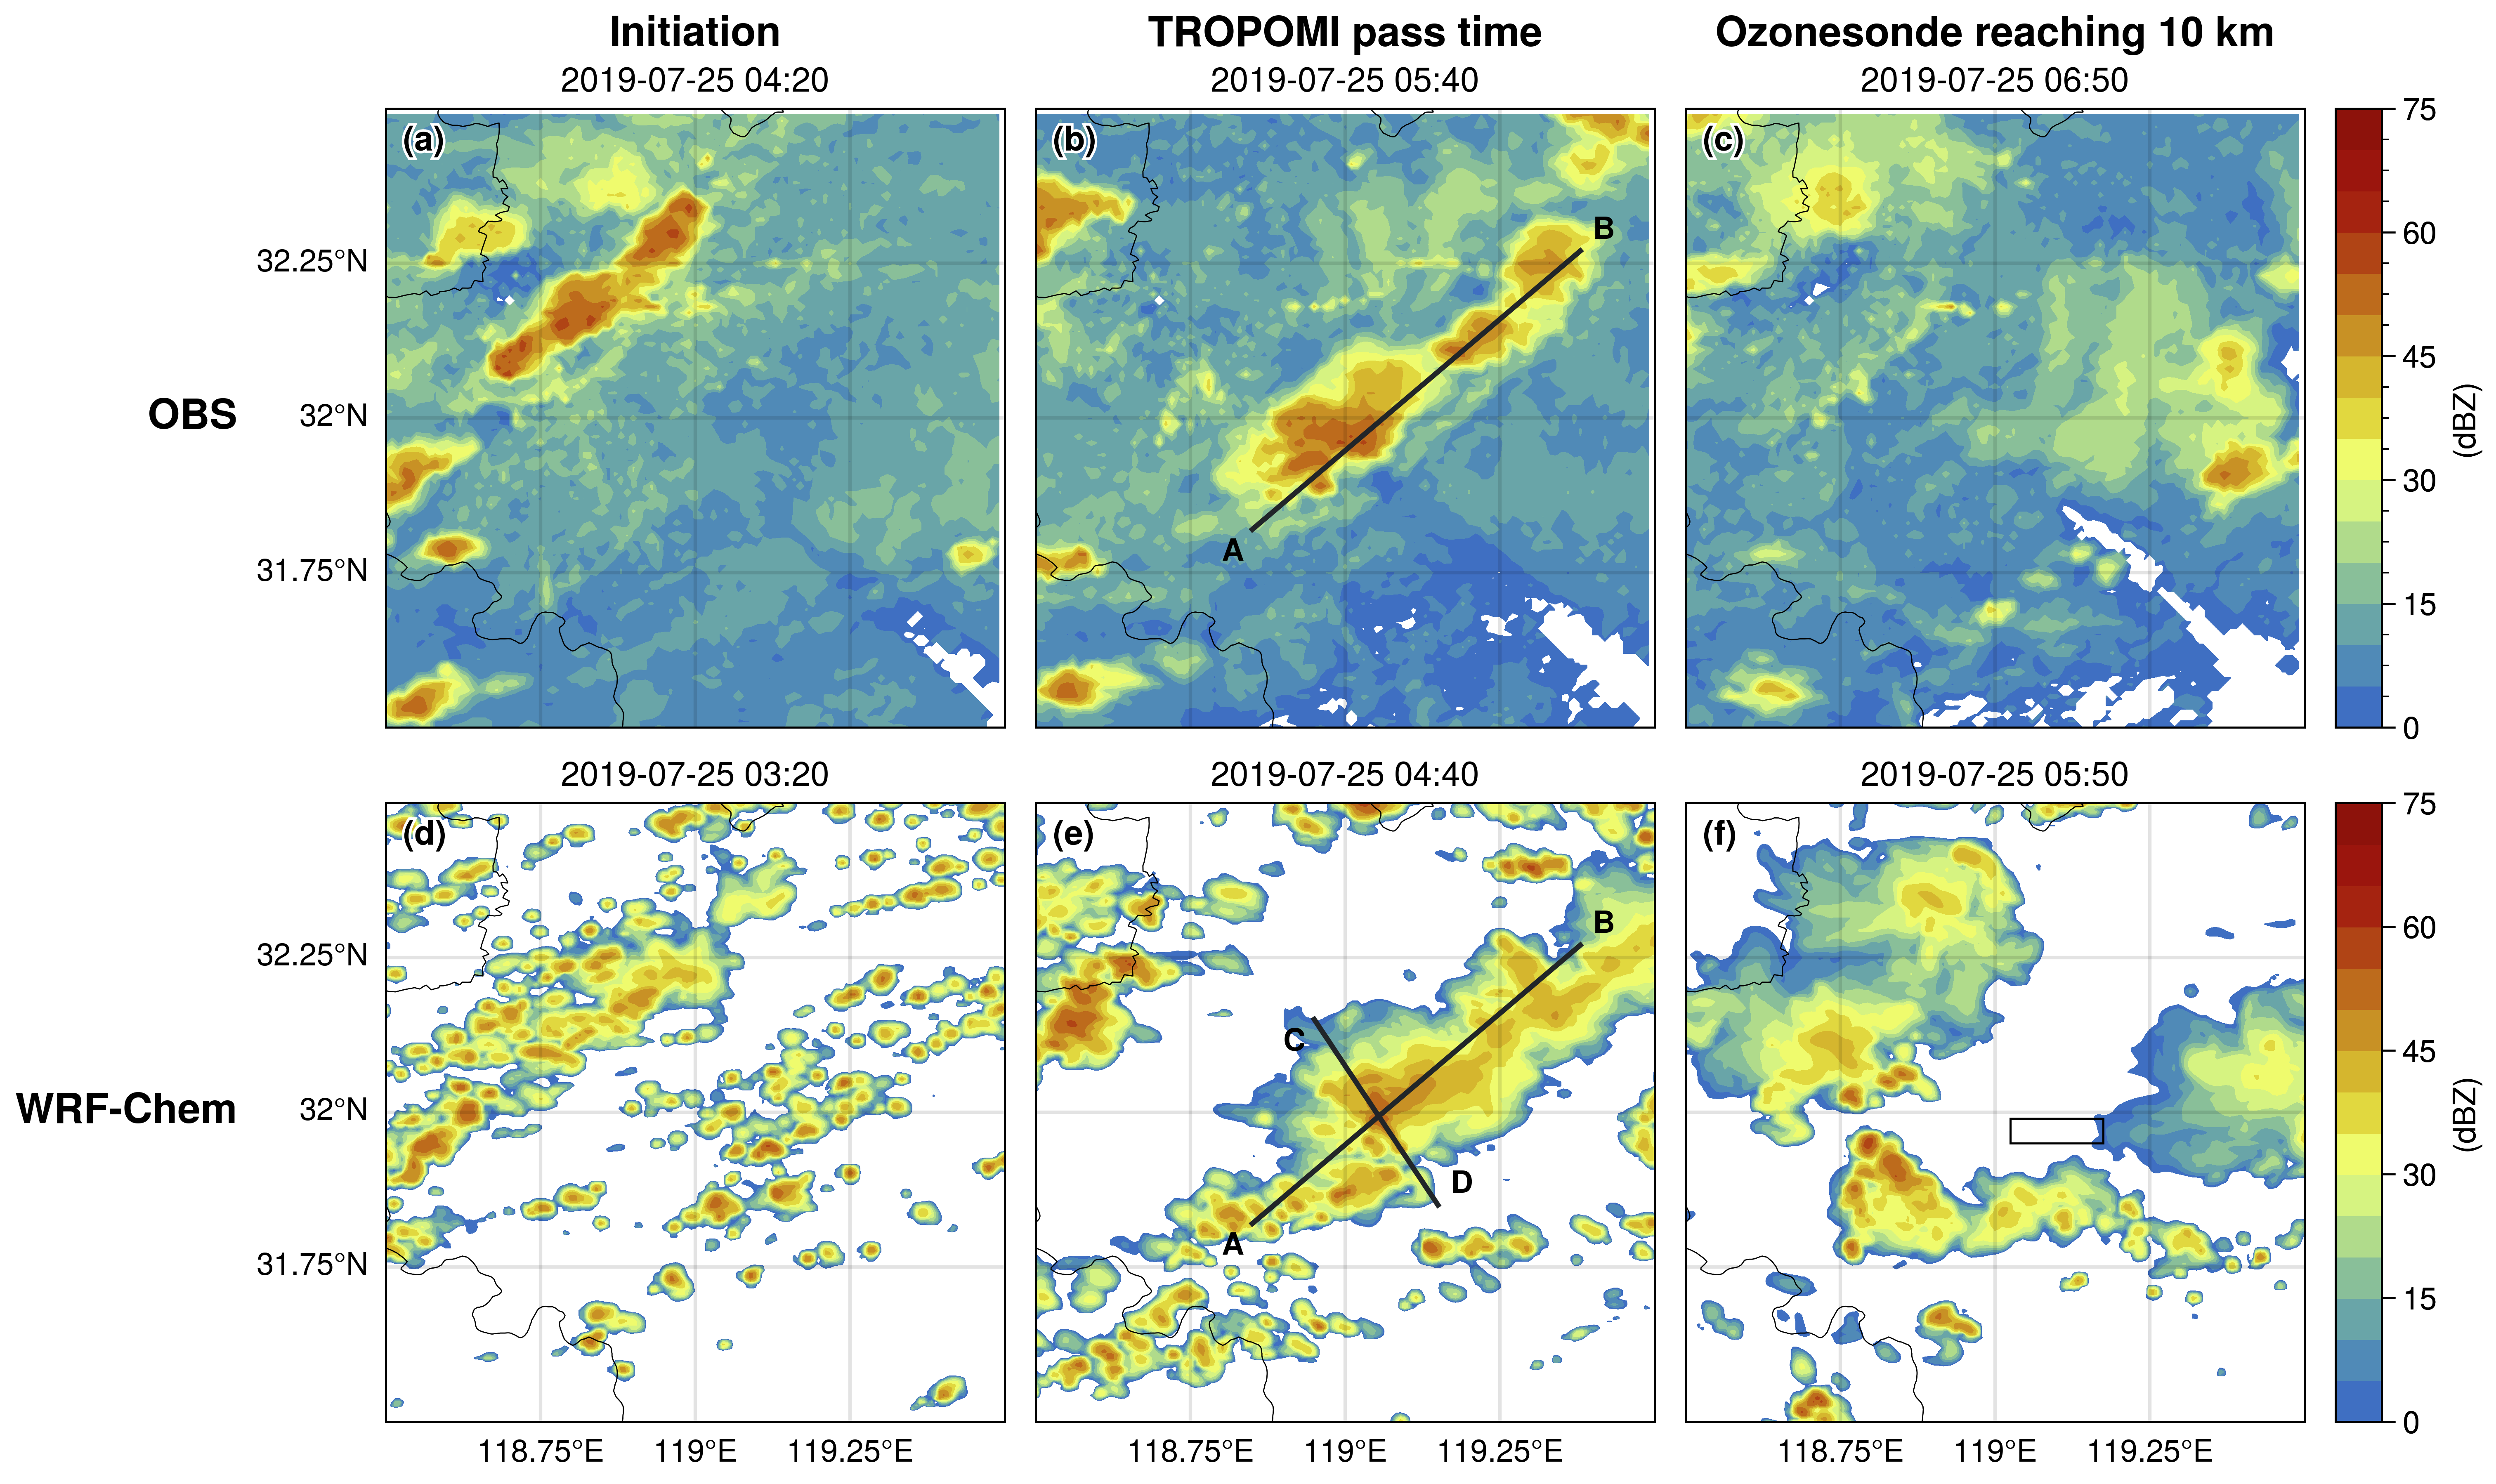
\includegraphics[width=\textwidth]{./figures/comp_crf_2019.png}
\caption{于(a)04:20 UTC、(b)05:40 UTC 和(c)06:50 UTC 观测到的雷达组合反射率;
         (d--e)WRF-Chem 在雷达观测时间前一小时模拟的雷达组合反射率;
         (b)和(e)中的 AB 实线是图 \ref{fig:comp_dbzcross_2019} 的剖面线;
         (e)中的CD实线是图\ref{fig:tendency_o3}b的剖面线。
         黑色矩形是与臭氧探空仪进行比较的区域。\\
         Figure \ref{fig:comp_crf_2019}. Observed radar composite reflectivity at (a) 04:20 UTC, (b) 05:40 UTC, and (c) 06:50 UTC.
        (d--e) WRF-Chem simulated composite reflectivity one hour before the radar observation times.
        The AB solid lines in (b) and (e) are cross section lines for Fig. \ref{fig:comp_dbzcross_2019}.
        The CD solid line in (e) is the cross section line for Fig. \ref{fig:tendency_o3}b.
        The black rectangle is the region for the comparison with ozonesonde.}
\label{fig:comp_crf_2019}
\end{figure}


与雷达观测相比,2019年7月25日和2020年9月1日模拟的对流初生时间,较实际情况分别提前了60和30分钟(图\ref{fig:comp_crf_2019}和图\ref{fig:comp_crf_2020}),闪电数据也以相同的时间间隔提前同化。
对于下文的结果比较,我们选择匹配的阶段而不是相同的时间。

2019年7月25日的热对流在初始时呈现为孤立的热泡,WRF-Chem再现了初始阶段孤立对流的位置和强度(图\ref{fig:comp_crf_2019}a和\ref{fig:comp_crf_2020}d)。
在05:40 UTC时,对流系统呈现东北--西南向,最大组合雷达反射率达到60 dBZ(图\ref{fig:comp_crf_2019}b),强度大于模拟的对流(最大组合雷达反射率为55 dBZ,图\ref{fig:comp_crf_2019}e)。
将模拟的对流核心区雷达反射率垂直剖面与观测结果进行对比(图\ref{fig:comp_dbzcross_2019}),
虽然对流距雷达过远造成缺失数据较多,但是在未进行人工插值的条件下,孤立对流的水平和垂直结构仍大致显示:
模拟的45 dBZ等值线达到12 km,但由于10 km 以上的数据质量低,
观测到的45 dBZ等值线仅达到10 km。

2020年9月1日观测到的飑线在北部初生,然后加强并向观测点移动(图\ref{fig:comp_crf_2020})。
对流旺盛阶段(最大组合雷达反射率为60 dBZ)大致在05:50 UTC,与TROPOMI过境时间相符(图\ref{fig:comp_dbzcross_2020}b,e)。
虽然该飑线抵达的最高高度低于2019年的热对流,但对流层低层(2--8 km)的反射率更大更广(图\ref{fig:comp_dbzcross_2020})。
由于模拟的对流消散区偏离了雷达观测的消散区,这导致与臭氧探空仪比较的区域设置在站点的西侧(图\ref{fig:comp_dbzcross_2020}c,f)。


\begin{figure}[H]
\centering
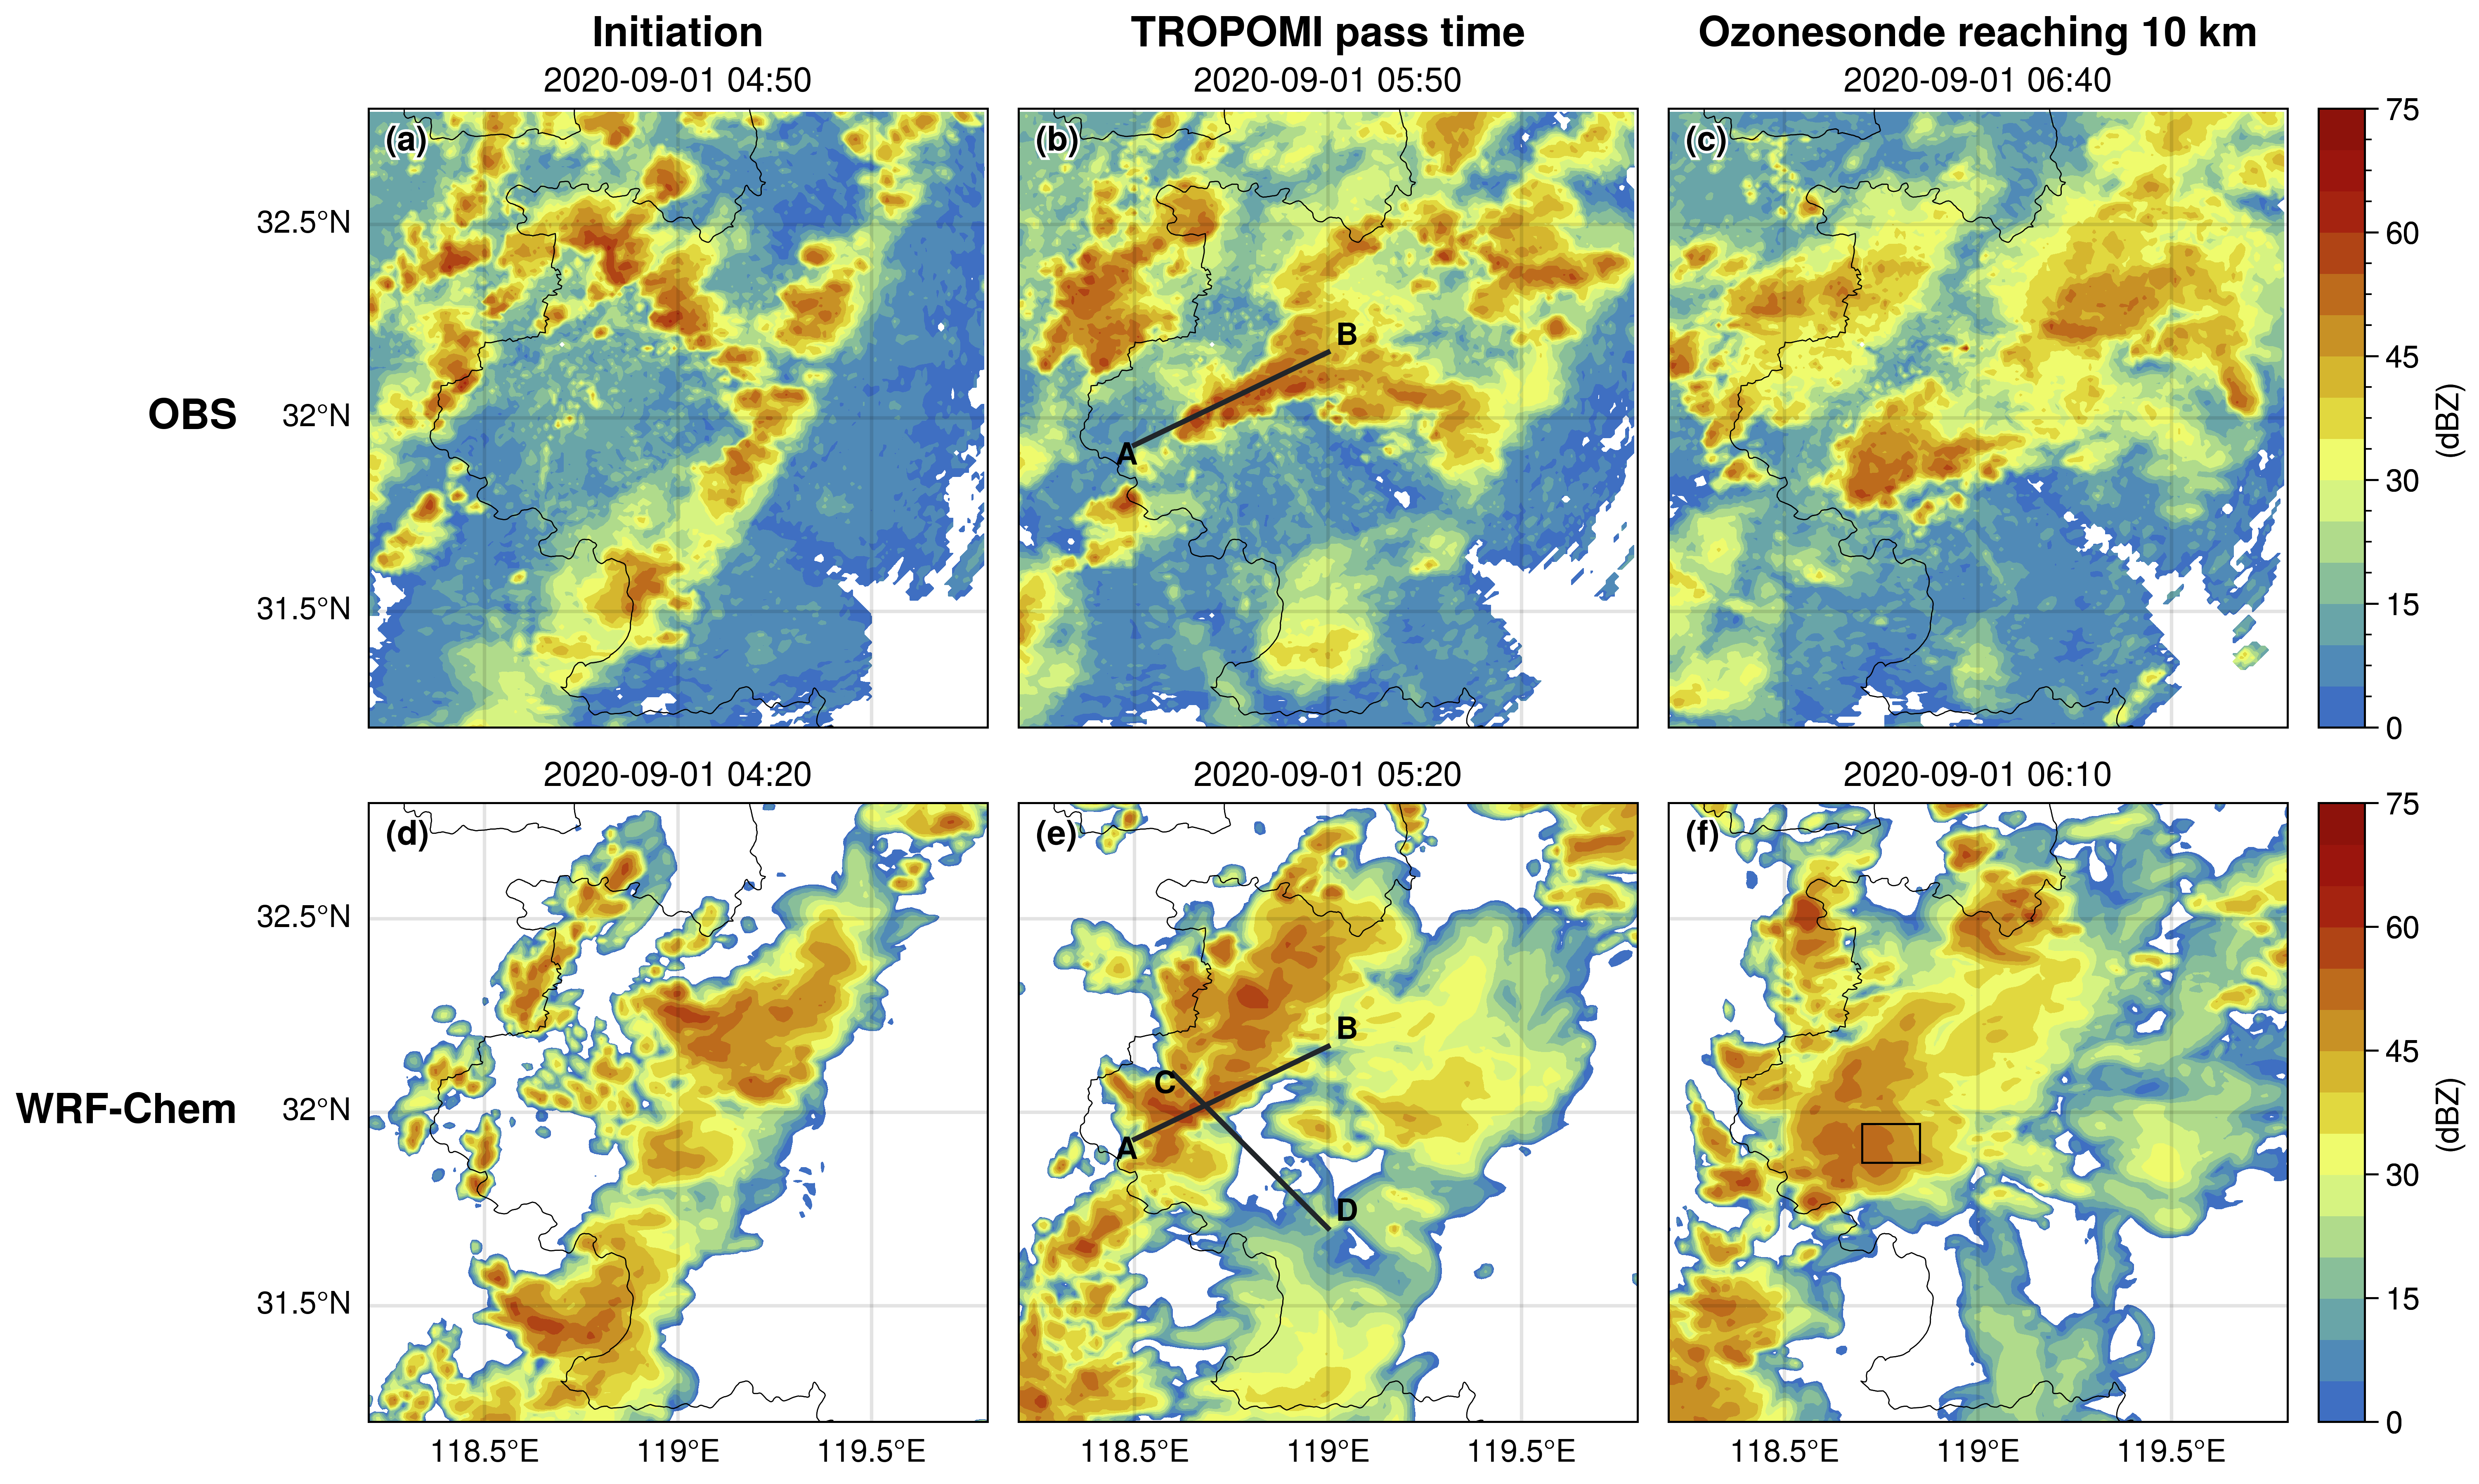
\includegraphics[width=\textwidth]{./figures/comp_crf_2020.png}
\caption{与图\ref{fig:comp_crf_2019} 相同,但针对2020年9月1日的对流个例,模拟时间比雷达观测提前30分钟。\\
Figure \ref{fig:comp_crf_2020}. Same as Fig. \ref{fig:comp_crf_2019} but for the case on 01 September 2020.
The simulation time is 30 minutes ahead of each radar observation.}
\label{fig:comp_crf_2020}
\end{figure}

\section{结果与讨论}

\subsection{臭氧的垂直分布} \label{sec:o3_profile}

如图\ref{fig:uto3_tropomi}所示,云切片方法可得到2019年6--8月中低纬度对流云不同高度O$_{\ch{3}}$的平均浓度,
其有效范围比NO$_{\ch{2}}$的云切片结果(图\ref{fig:utno2_tropomi})更广,
尤其是在中云和高云条件下的中纬度地区(图\ref{fig:uto3_tropomi}b--d)。
这是由于TROPOMI的O$_{\ch{3}}$二级产品中云分数为光学云识别算法(OCRA)云分数,而NO$_{\ch{2}}$二级产品中使用从氧气A波段版本S(FRESCO-S)中快速检索云的方案。


\begin{figure}[H]
\centering
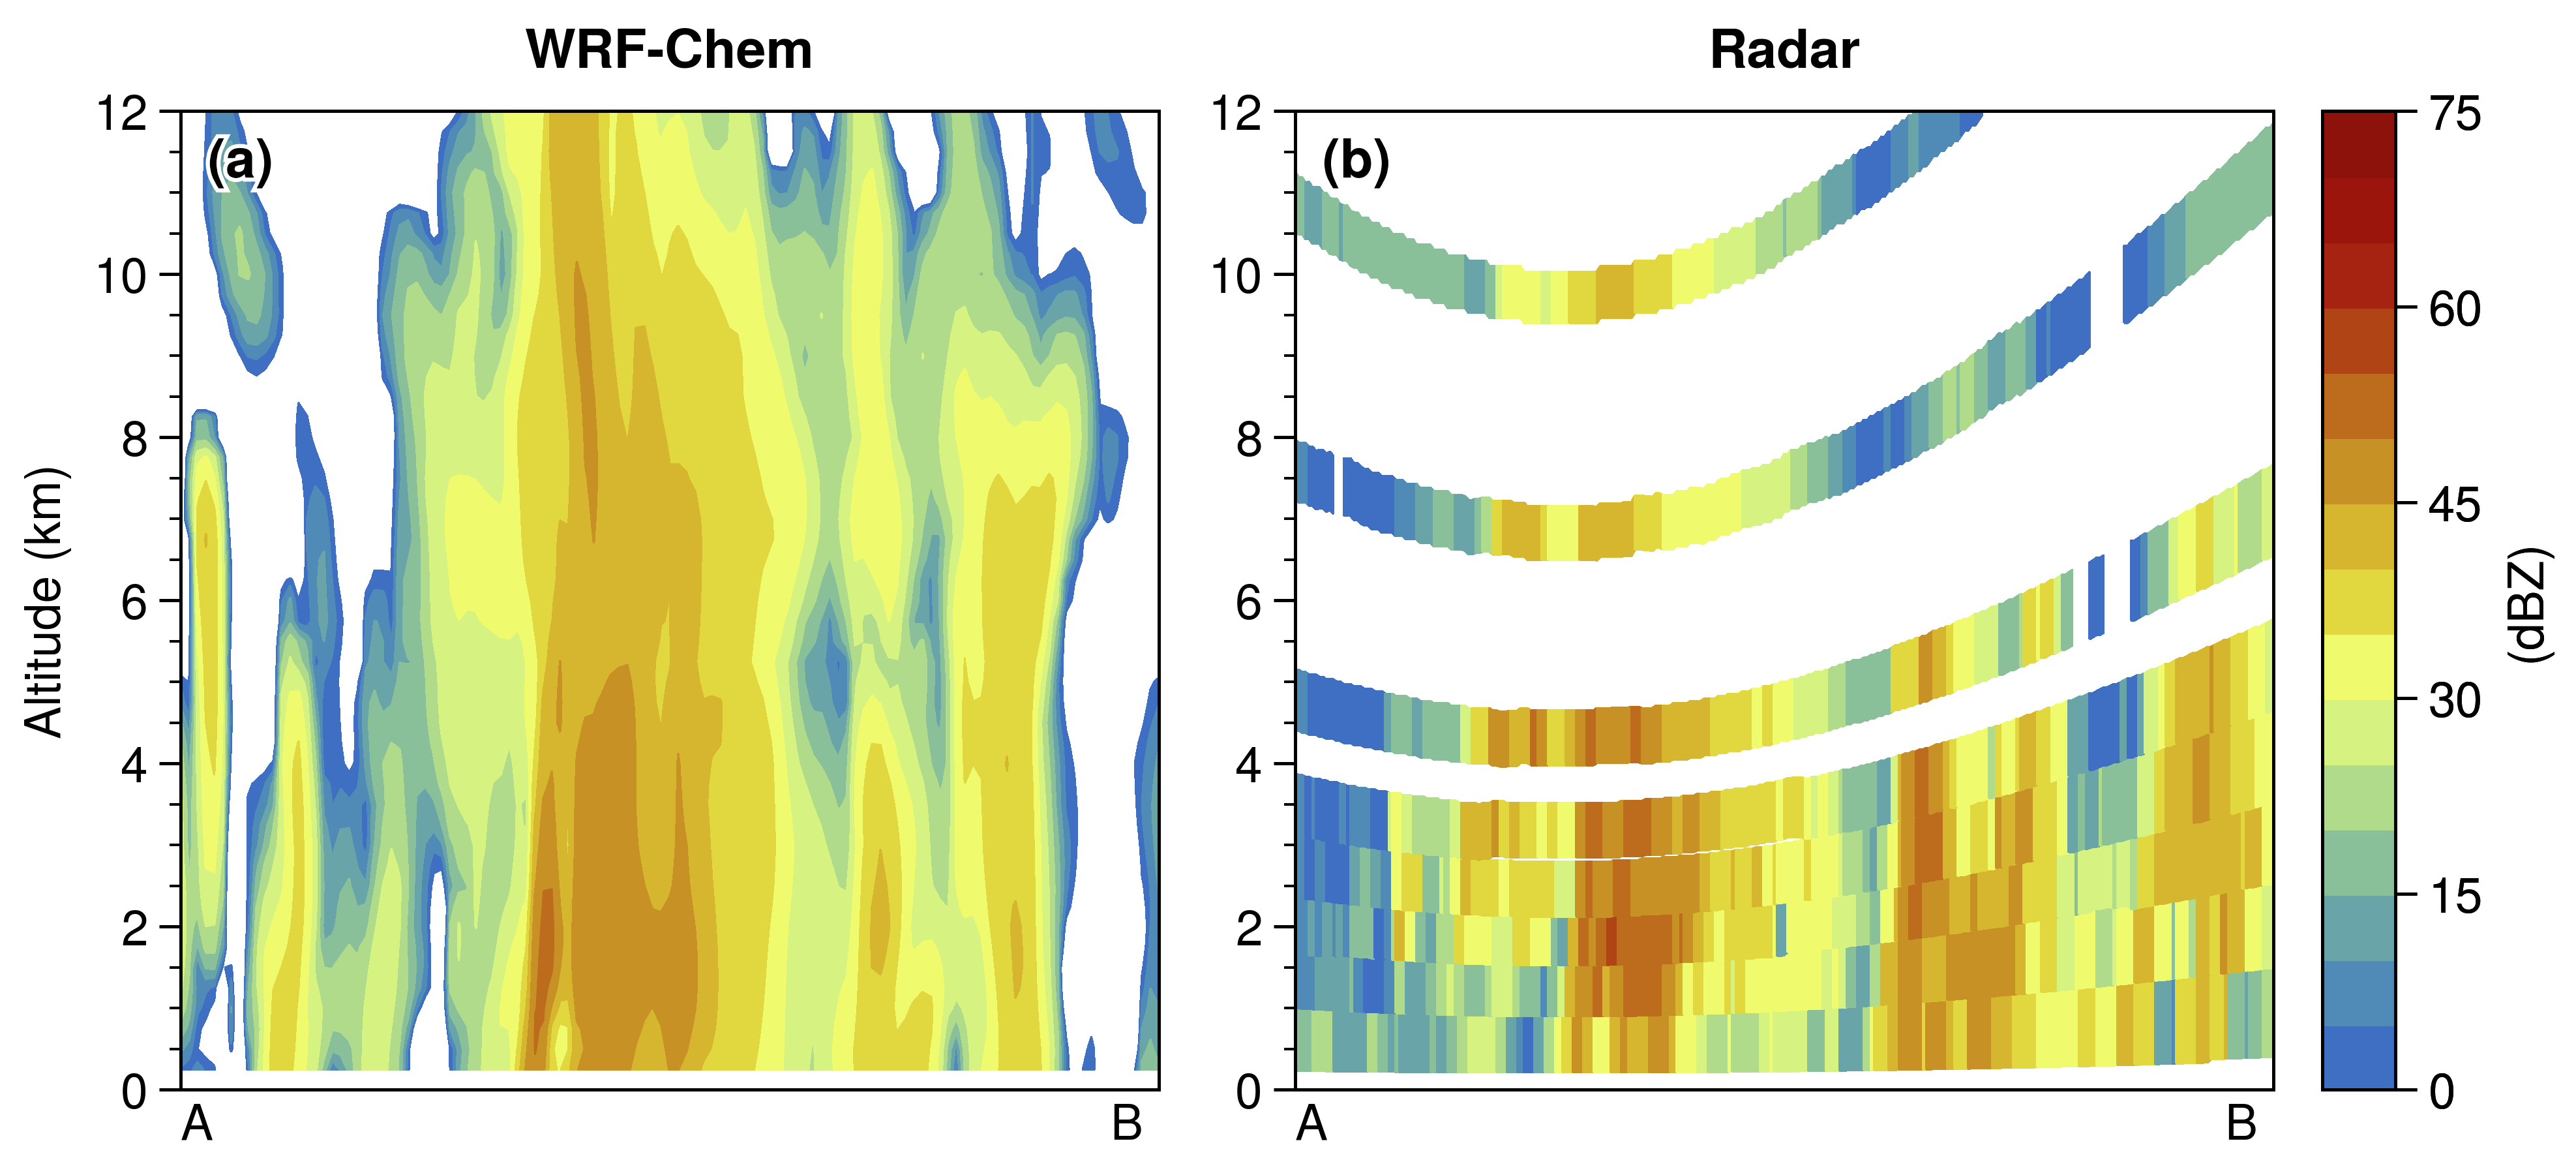
\includegraphics[width=0.9\textwidth]{./figures/comp_dbzcross_2019.png}
\caption{沿着图\ref{fig:comp_crf_2019}中AB线剖得的2019年7月25日(a)WRF-Chem模拟和(b)雷达观测的雷达反射率。\\
Figure \ref{fig:comp_dbzcross_2019}. Vertical cross sections of (a) WRF-Chem simulated and (b) observed radar reflectivity fields along the transect lines (AB) in Fig. \ref{fig:comp_crf_2019} for 25 July, 2019.}
\label{fig:comp_dbzcross_2019}
\end{figure}

\begin{figure}[H]
\centering
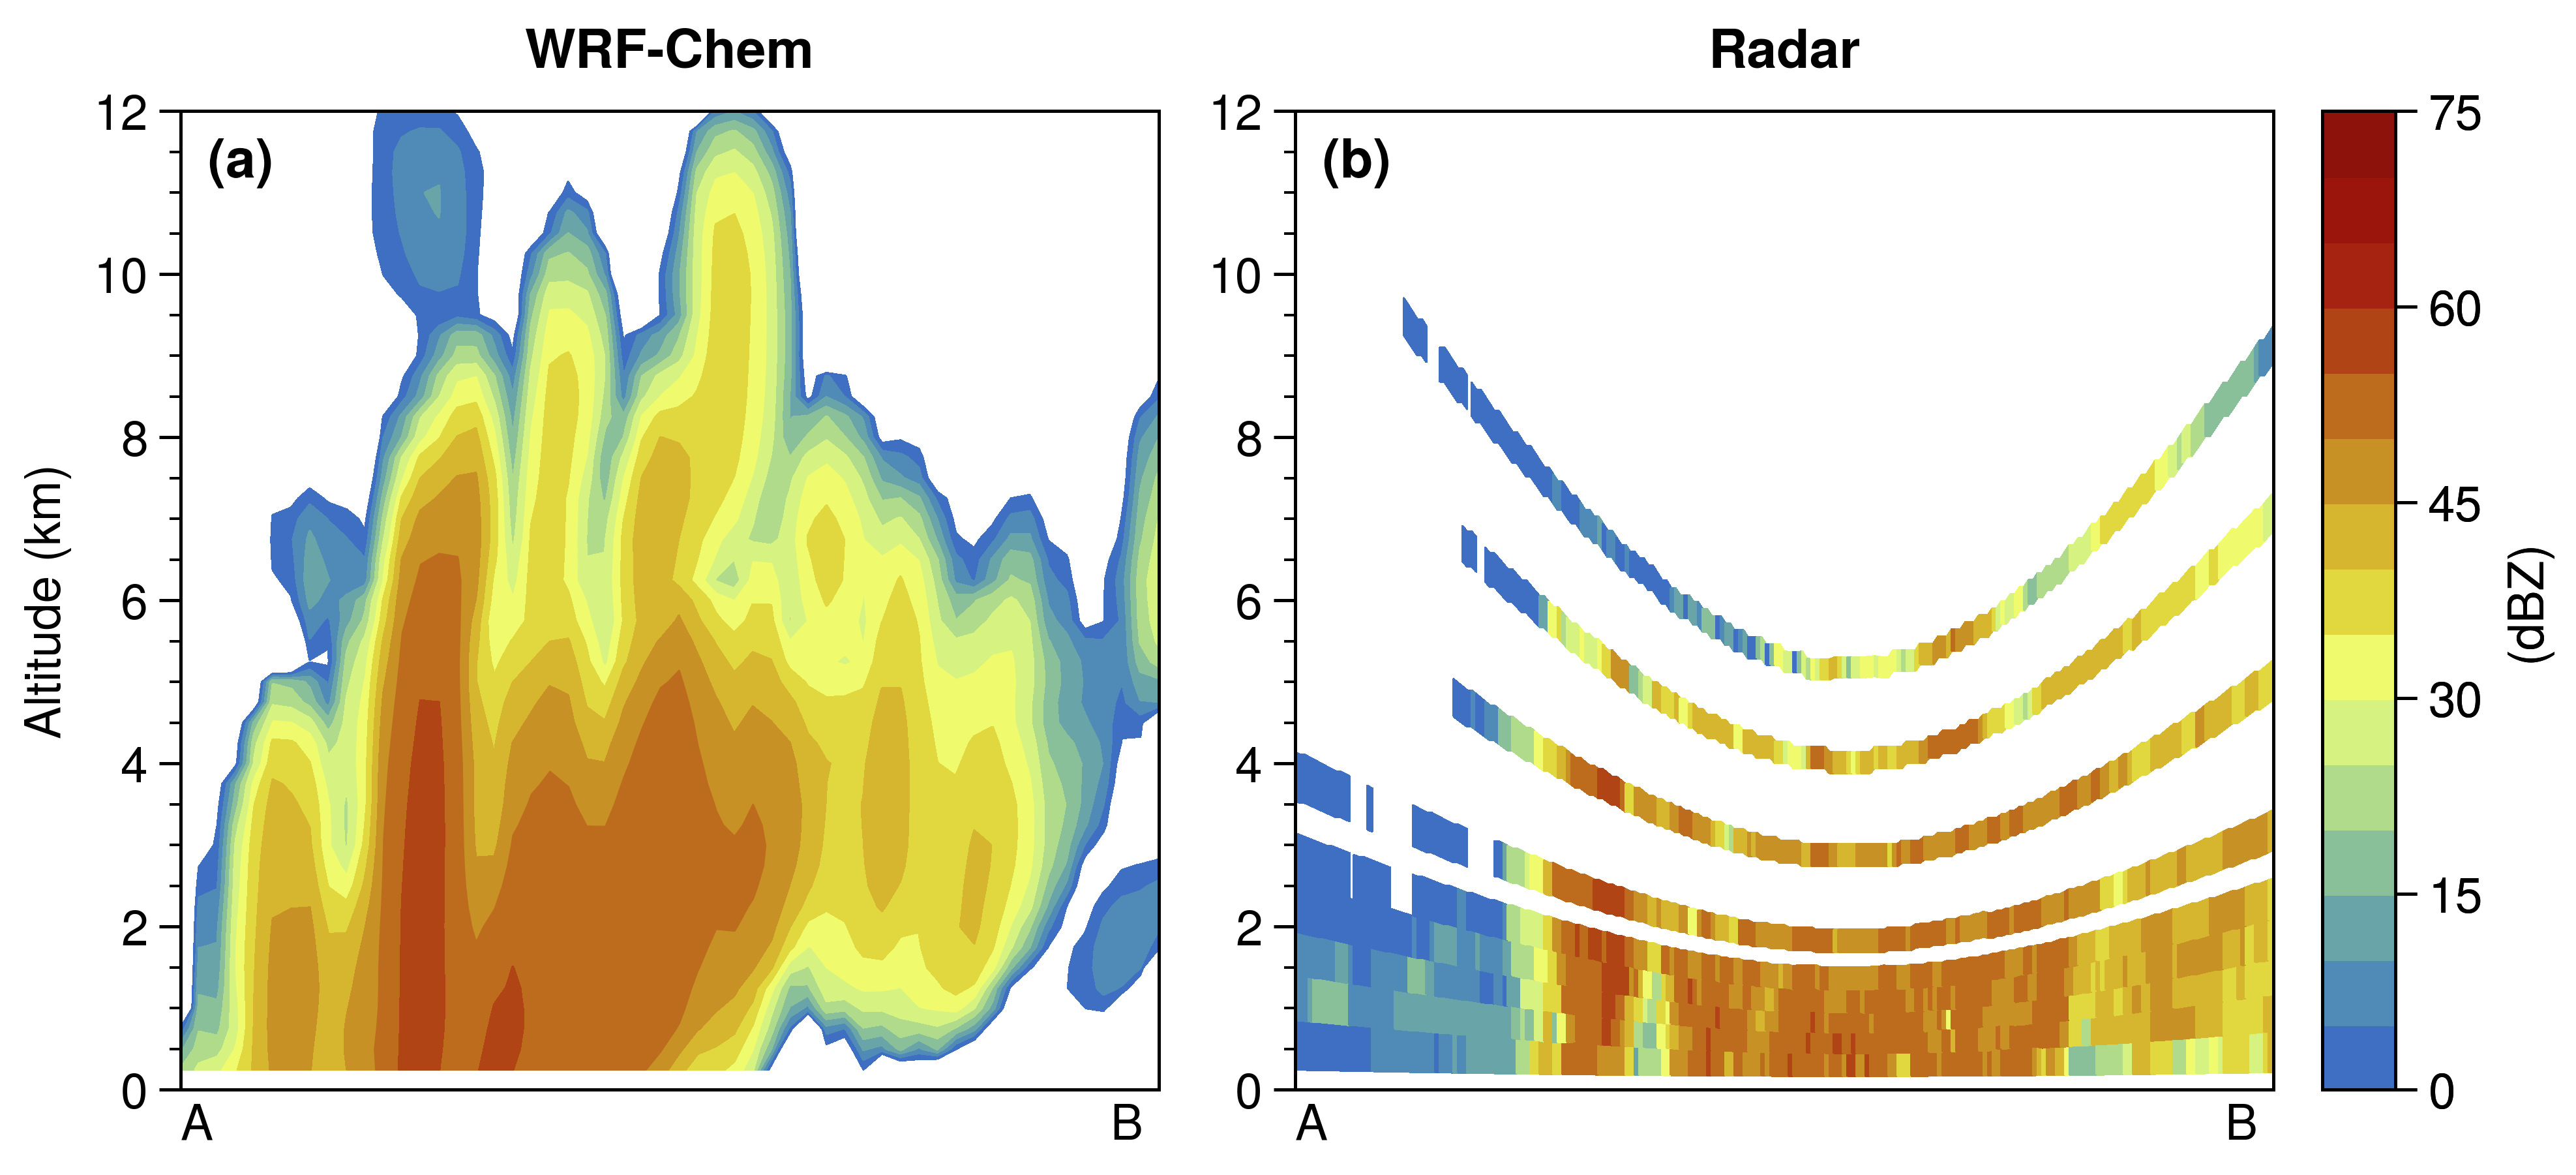
\includegraphics[width=0.9\textwidth]{./figures/comp_dbzcross_2020.png}
\caption{与图\ref{fig:comp_dbzcross_2019}相同,但针对2020年9月1日的对流个例。\\
Figure \ref{fig:comp_dbzcross_2020}. Same as Figure \ref{fig:comp_dbzcross_2019} but for the case on 01 September 2020.}
\label{fig:comp_dbzcross_2020}
\end{figure}

总体来看,高云处的O$_{\ch{3}}$浓度(图\ref{fig:uto3_tropomi}a--b)高于中云(图\ref{fig:uto3_tropomi}c--d),
其中对流层顶--330 hPa间的O$_{\ch{3}}$为330--450 hPa间的$\sim$1.5倍,为450--570 hPa间的$\sim$2倍。
对于热带地区,非洲中部(20$^{\circ}$ W--50$^{\circ}$ E,0--20$^{\circ}$ N)的O$_{\ch{3}}$浓度比同纬度地区的O$_{\ch{3}}$浓度高,尤其是在中云和高云条件下可高出40--48\%,该现象与\citet{Cooper.2013}研究中215 hPa高度MLS的O$_{\ch{3}}$观测结果相符。
他们的研究指出,低O$_{\ch{3}}$事件经常发生在热带西太平洋,很少发生在热带其他地区,
而热带海洋区域在低O$_{\ch{3}}$事件和高云的频率之间存在一致的空间特征,表明这些事件来自于对流。
虽然非洲中部也是强对流频发地区,但生物质燃烧导致陆地边界层O$_{\ch{3}}$浓度往往高于海洋\citep{Thompson.2001,Anderson.2016},因此深对流产生较少的低O$_{\ch{3}}$事件。

\begin{figure}[H]
    \centering
    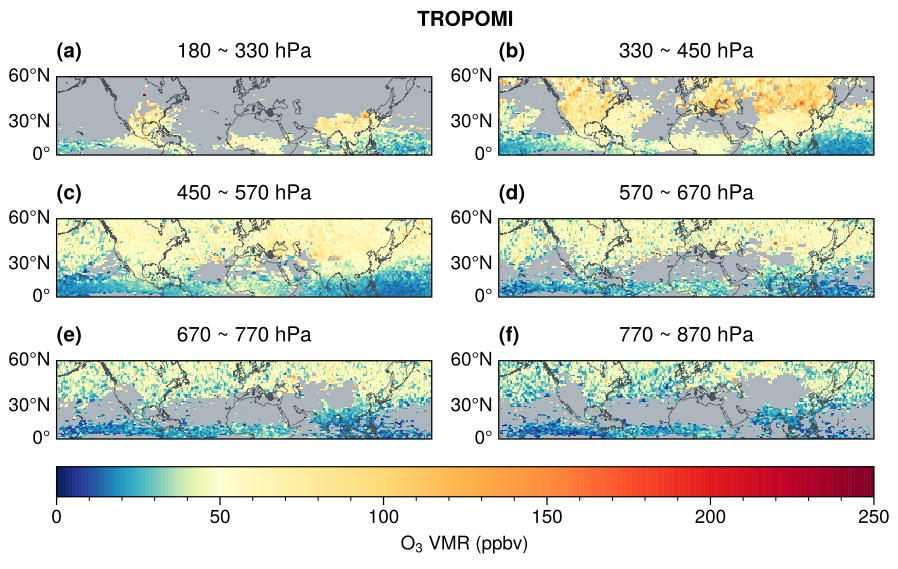
\includegraphics[width=0.95\textwidth]{./figures/uto3_tropomi.png}
    \caption{
    TROPOMI云切片算法所得的2019年6--8月北半球中低纬度O$_{\ch{3}}$浓度分布图。 \\
    Figure \ref{fig:uto3_tropomi}. The O$_{\ch{3}}$ vertical mixing ratios derived from the cloud-slicing results of TROPOMI O$_{\ch{3}}$ observations at the northern middle-low latitudes for June--August in 2019.
    }
    \label{fig:uto3_tropomi}
\end{figure}

为了进一步利用MERRA2-GMI的模式结果分析动力输送和化学反应在其中的作用,我们首先将各个高度的MERRA2-GMI模式结果与TROPOMI观测数据相比较。
图\ref{fig:uto3_merra2}为2019年6--8月与TROPOMI对应的MERRA2-GMI O$_{\ch{3}}$模拟结果,
图\ref{fig:uto3_delta}为TROPOMI与MERRA2-GMI在各层的结果之差($\Delta$ O$_{\ch{3}}$)。
总体上,非洲中部的$\Delta$ O$_{\ch{3}}$在中云和高云条件下为负(-23 $\pm$ 11 pptv,图\ref{fig:uto3_delta}a--d),
中纬度陆地地区的$\Delta$ O$_{\ch{3}}$在高云条件下为正(20 $\pm$ 15 pptv,图\ref{fig:uto3_delta}b)。
此外,$\Delta$ NO$_{\ch{2}}$(图\ref{fig:utno2_tropomi})和$\Delta$ O$_{\ch{3}}$(图\ref{fig:uto3_delta})的对比显示,
尽管中云和高云条件下NO$_{\ch{2}}$在大部分陆地地区被高估,但是O$_{\ch{3}}$却被低估。
\citet{Pickering.1990}于美国中南部清洁地区的研究显示,11 km处的LNO峰值排放导致该高度层为VOC控制区。
由于本研究全球模式中除化学反应外,动力输送也存在偏差,故不能确定是否为VOC控制区,有待将来进一步的研究。
低云条件下云切片算法低估O$_{\ch{3}}$的现象,也反映了AMF$_{\ch{geo}}$在低云和污染条件下的高估\citep{BelmonteRivas.2015}。


\begin{figure}[H]
    \centering
    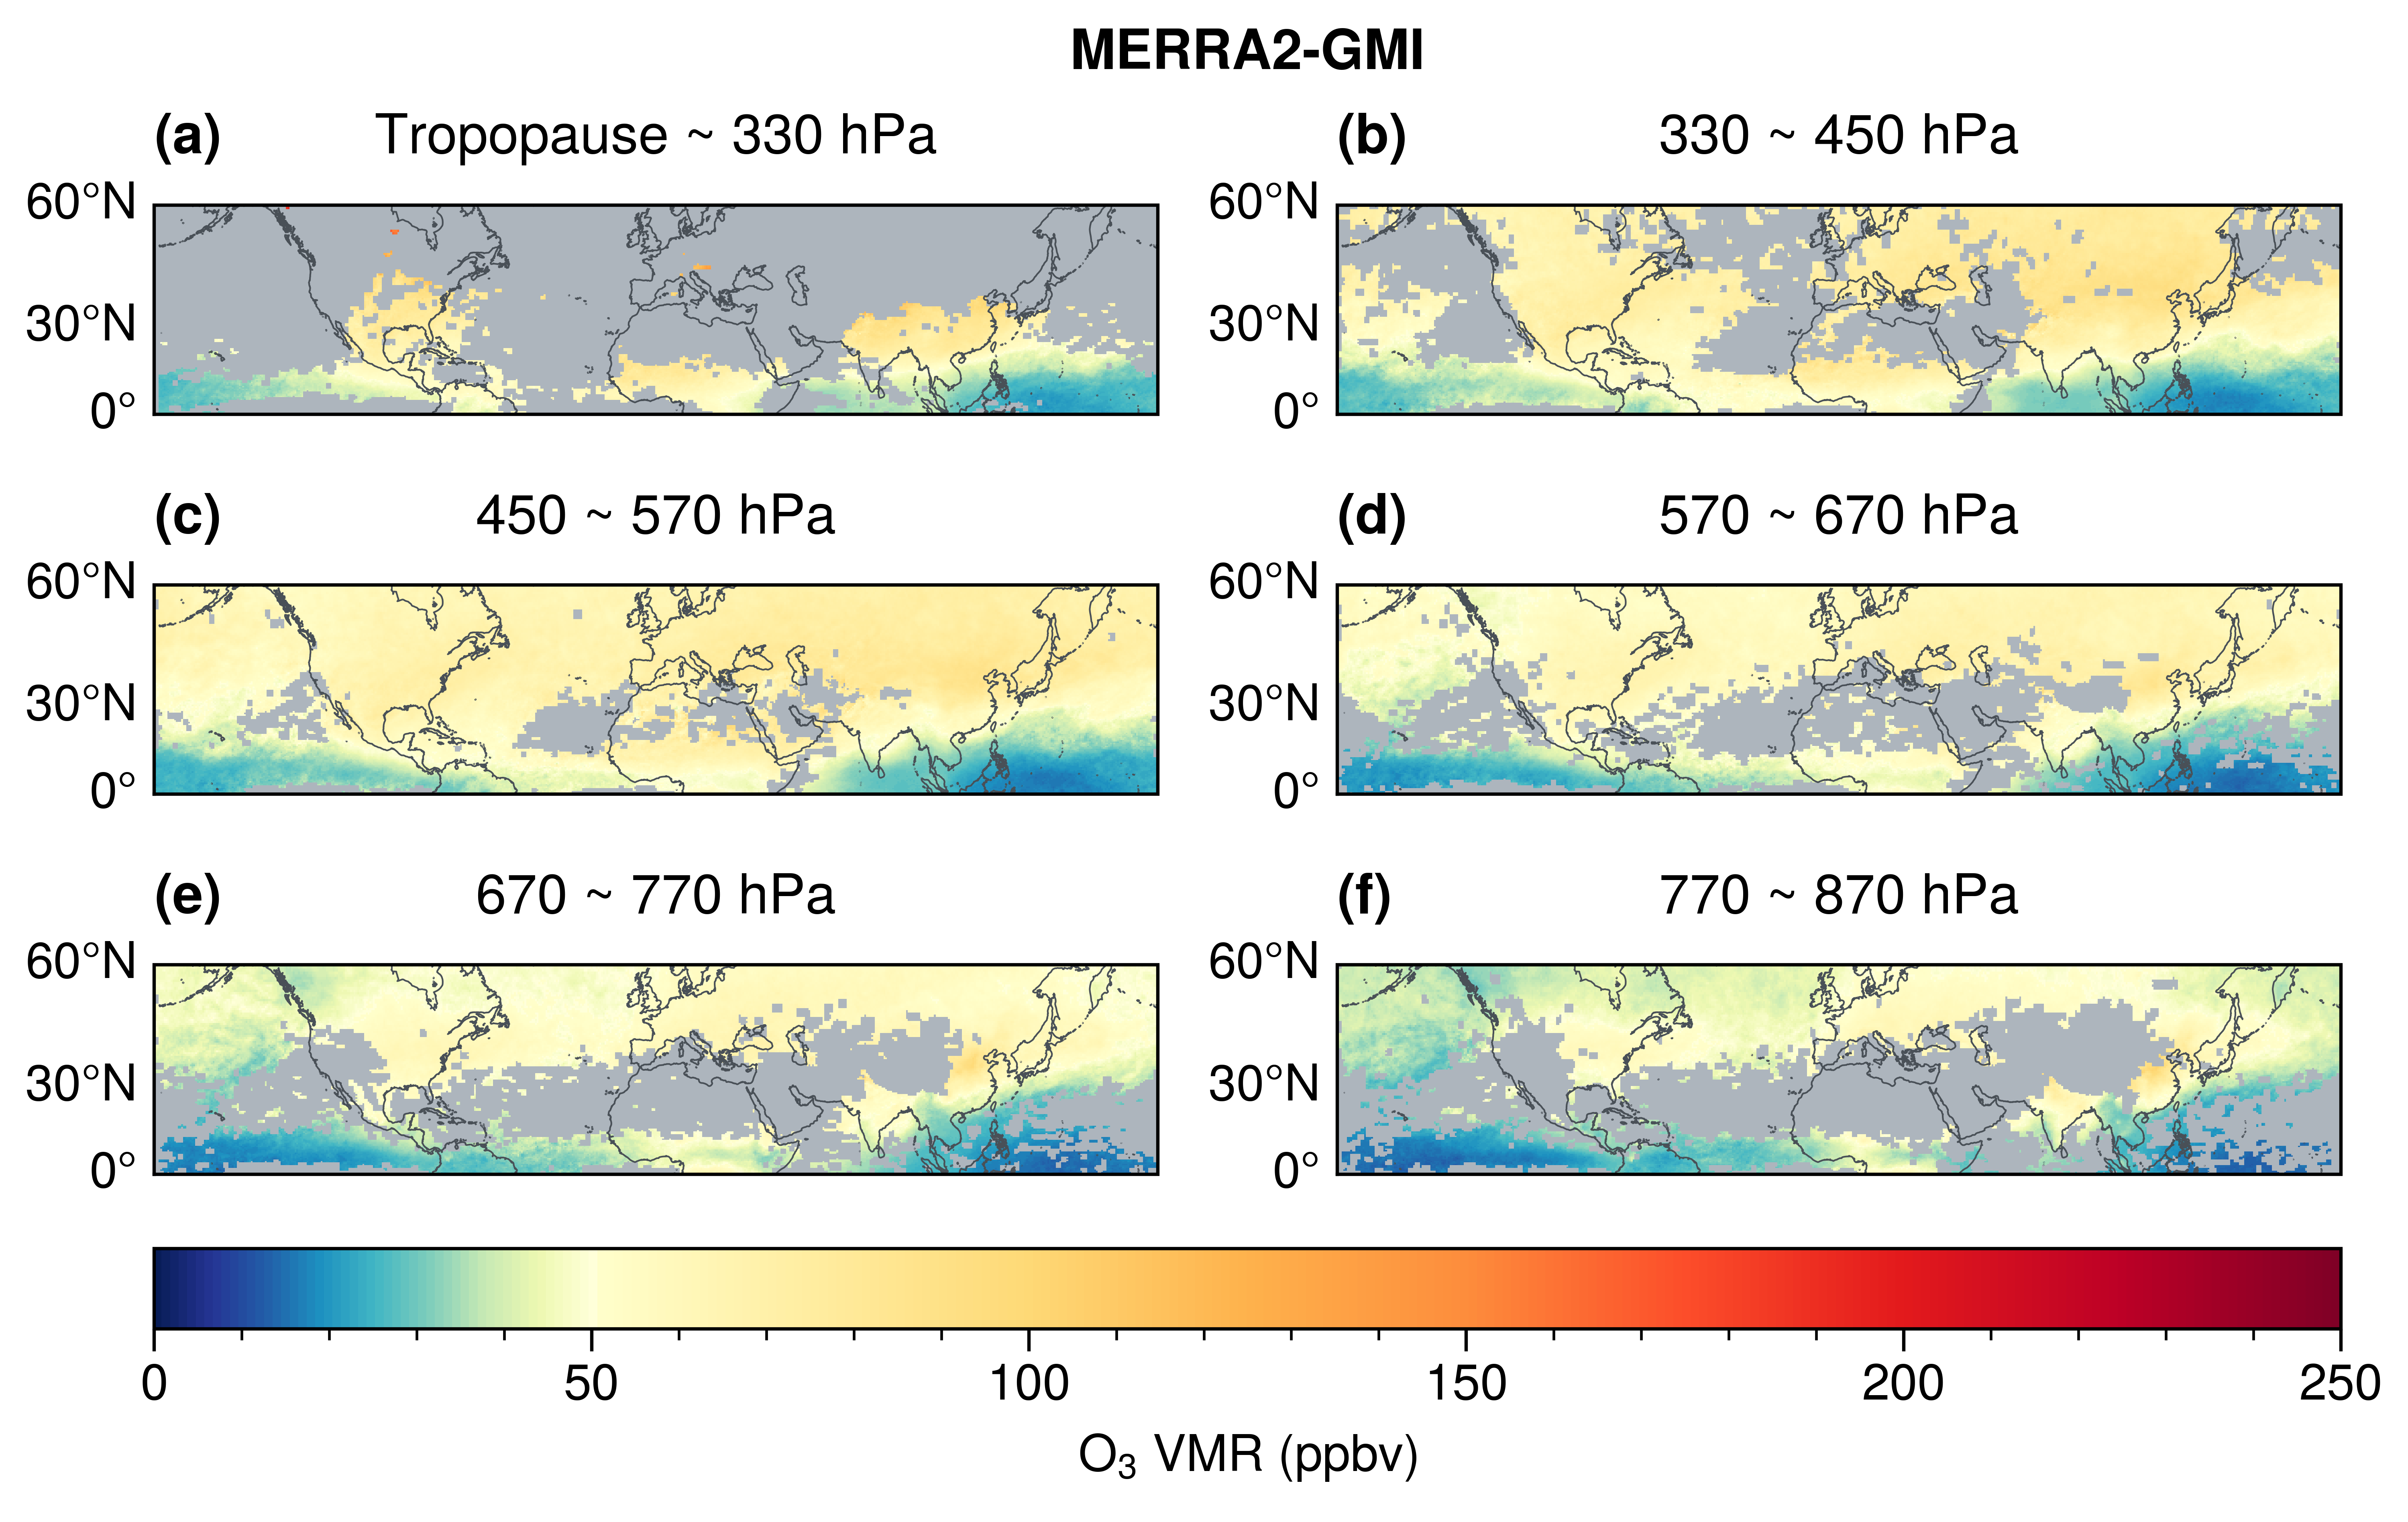
\includegraphics[width=0.9\textwidth]{./figures/uto3_merra2-gmi.png}
    \caption{
    同图\ref{fig:uto3_tropomi}但数据为MERRA2-GMI。 \\
    Figure \ref{fig:uto3_merra2}. Same as Fig. \ref{fig:uto3_tropomi} but for MERRA2-GMI.
    }
    \label{fig:uto3_merra2}
\end{figure}


\begin{figure}[H]
    \centering
    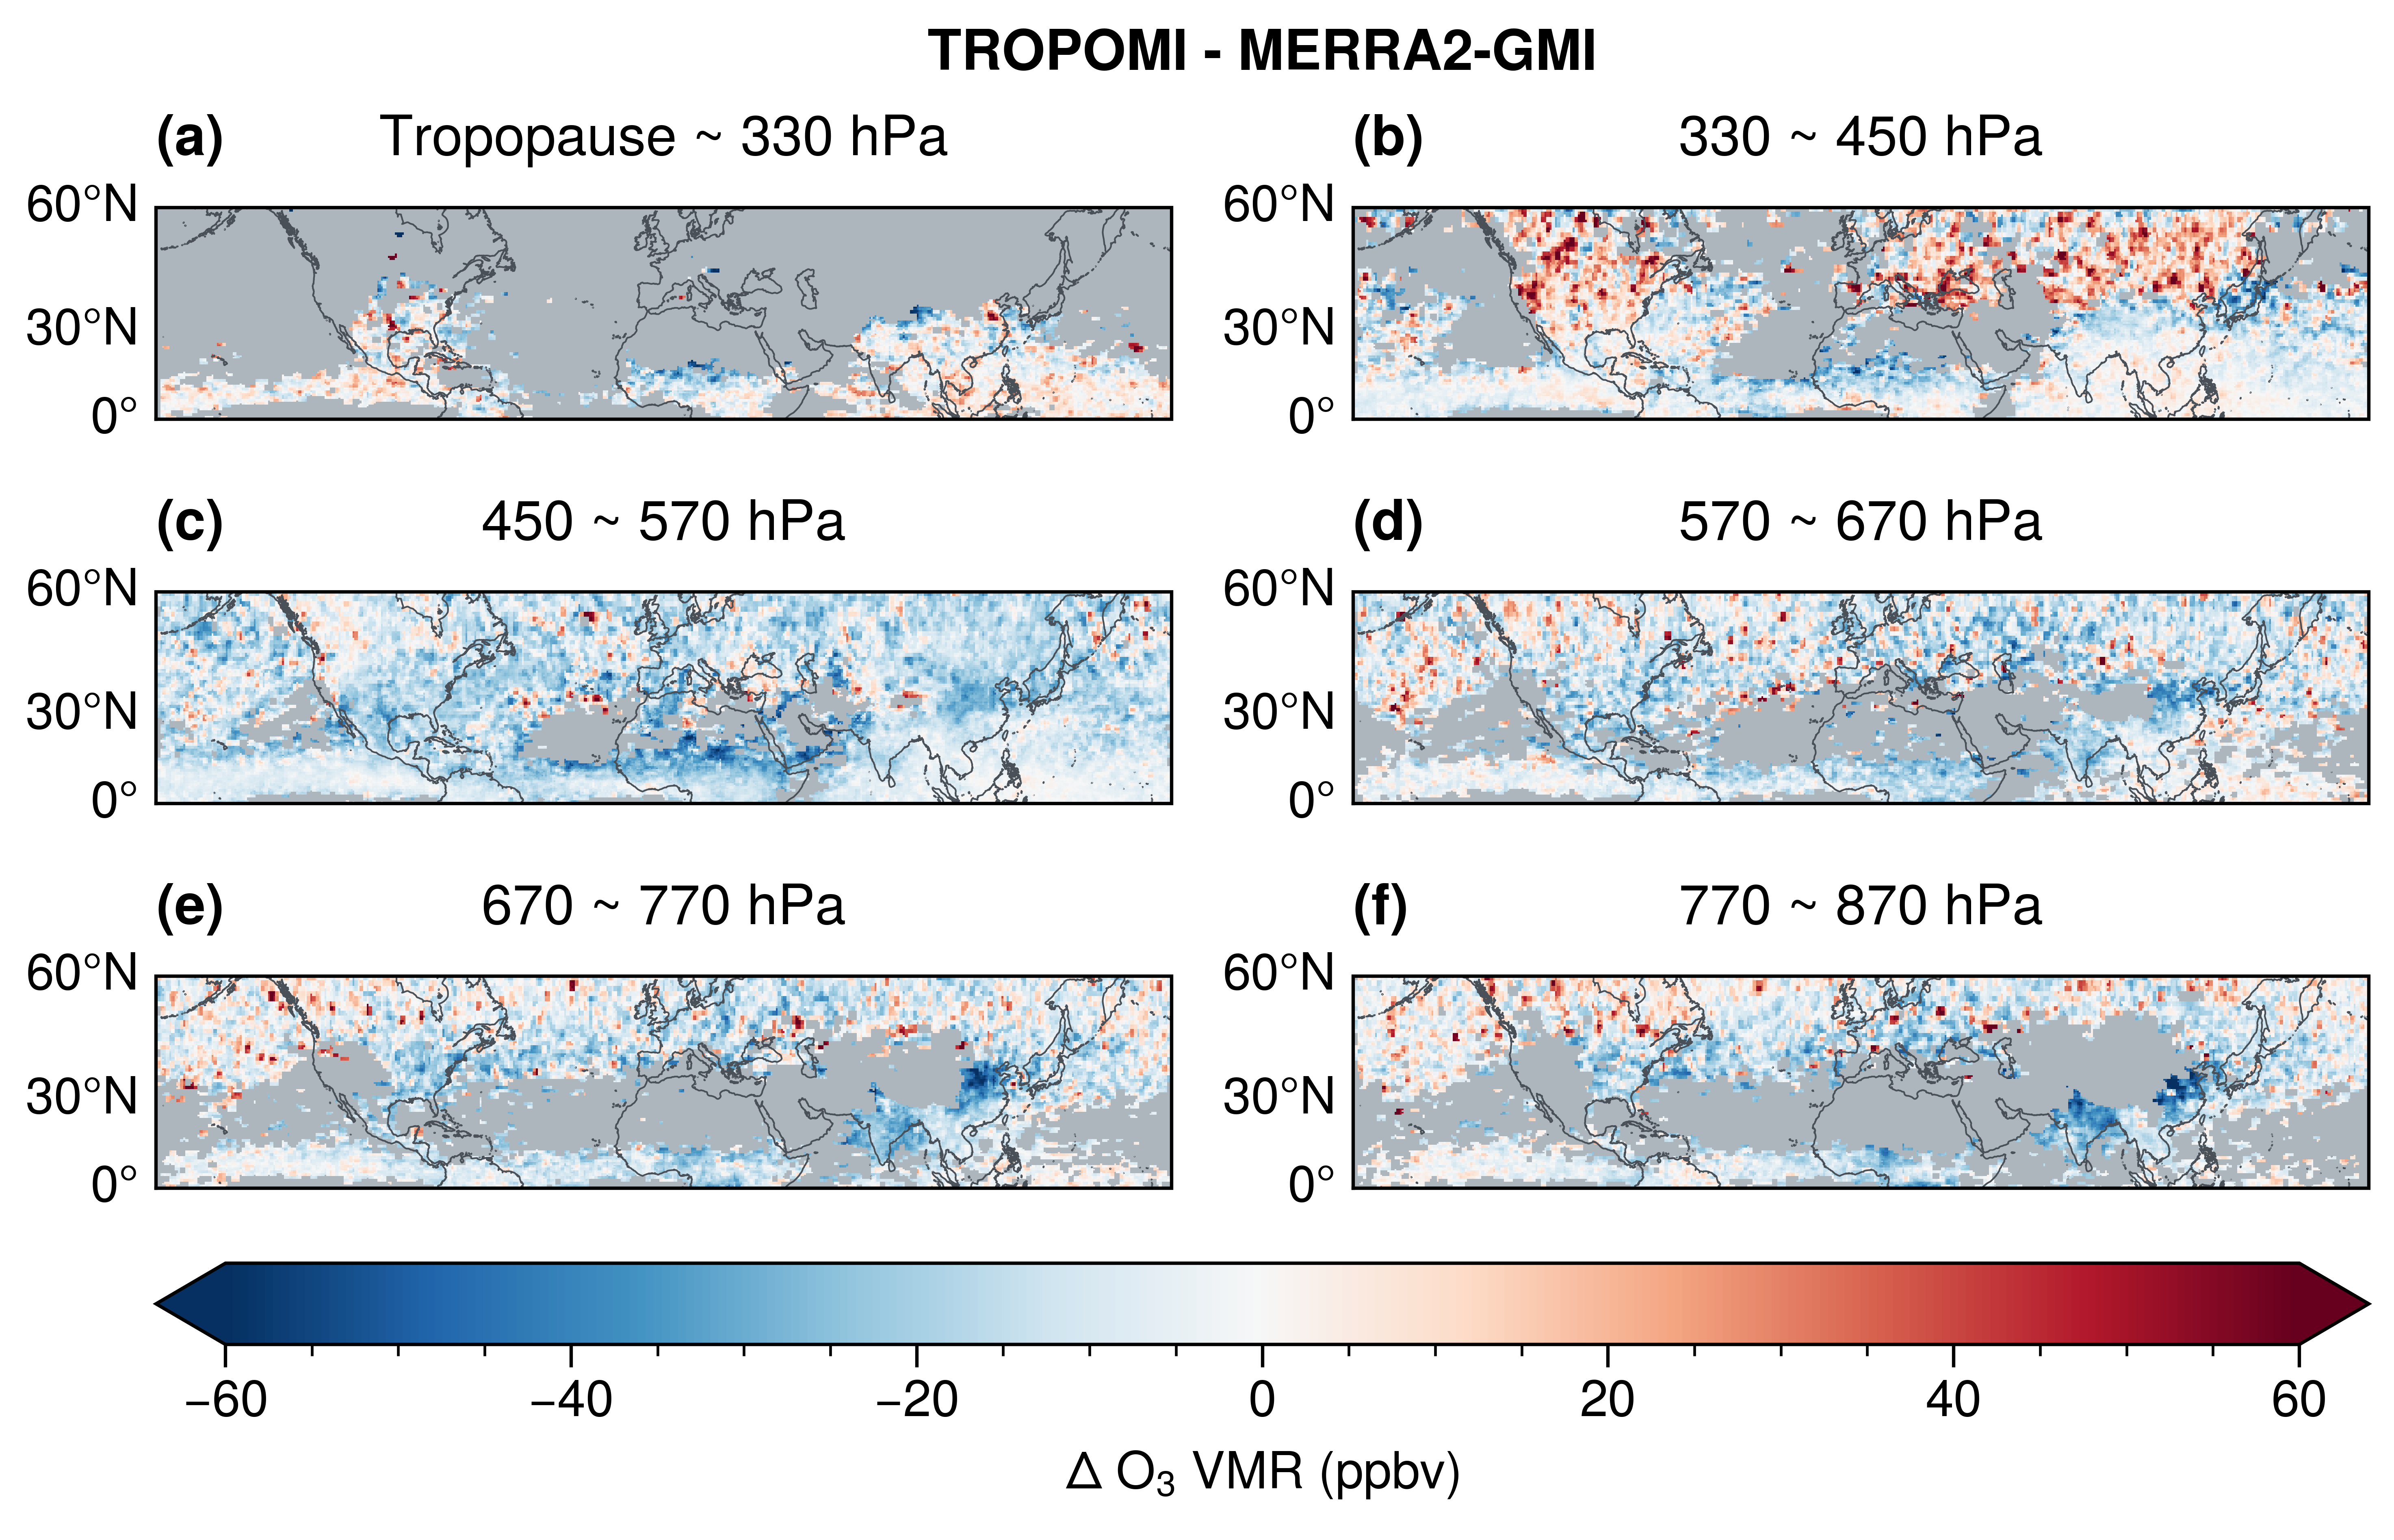
\includegraphics[width=0.9\textwidth]{./figures/uto3_delta.png}
    \caption{
    图\ref{fig:uto3_tropomi}与图\ref{fig:uto3_merra2}之差。 \\
    Figure \ref{fig:uto3_delta}. Differences between Fig. \ref{fig:uto3_tropomi} and Fig. \ref{fig:uto3_merra2}.
    }
    \label{fig:uto3_delta}
\end{figure}


鉴于高云条件下的云切片结果在中纬度地区有效数较少(图\ref{fig:uto3_tropomi}a),
我们将MLS于261 hPa高度观测的O$_{\ch{3}}$浓度与MERRA2-GMI的O$_{\ch{3}}$模拟结果,在晴空和有云条件下分别进行对比。
如图\ref{fig:mls_o3_261hpa}所示,在低纬度地区两者均显示有云条件下海洋上O$_{\ch{3}}$平均浓度较晴空降低17\%,非洲中部和印度北部的O$_{\ch{3}}$平均浓度较晴空增大20\%。
虽然晴空条件下两者在中纬度地区的O$_{\ch{3}}$浓度一致,但有云时两者的变化相反。
具体而言,MLS观测显示有云条件下中纬度地区261 hPa高度的O$_{\ch{3}}$平均浓度比晴空时的浓度高24\%,
而MERRA2-GMI模拟结果显示O$_{\ch{3}}$平均浓度比晴空时低26\%。
在40--60$^{\circ}$ N区域内有高云的条件下,MERRA2-GMI模拟的O$_{\ch{3}}$平均浓度为108 ppbv,与同范围内TROPOMI云切片得到的O$_{\ch{3}}$平均浓度(86 ppbv)相接近,而MLS的平均观测结果(230 ppbv)为MERRA2-GMI和TROPOMI的2--3倍。
由于MLS的O$_{\ch{3}}$廓线在对流层上层的分辨率为3--6 km,而261 hPa所在高度接近中纬度地区的对流层顶,故过度的外推可能导致MLS测得的O$_{\ch{3}}$浓度过高\citep{Schoeberl.2007}。


\begin{figure}[H]
    \centering
    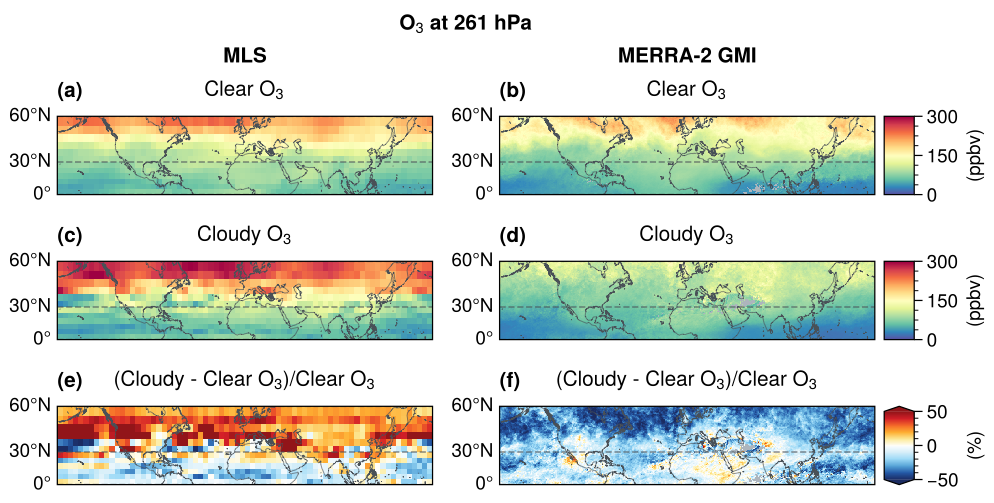
\includegraphics[width=\textwidth]{./figures/mls_o3_261hpa.png}
    \caption{
    2019年6--8月北半球中低纬度晴空(a--b)和有云(c--d)条件下261 hPa高度O$_{\ch{3}}$的平均浓度,以及相对百分比变化(e--f)。
    第一列为MLS观测数据,第二列为MERRA2-GMI模拟结果。 \\
    Figure \ref{fig:mls_o3_261hpa}. The mean O$_{\ch{3}}$ concentrations at 261 hPa with clear (a--b) and cloudy (c--d) conditions at the northern middle-low latitudes for June--August in 2019. The percentage differences are shown in panel (e) and (f).
    The first column is the MLS observations while the second column is the MERRA2-GMI simulations.
    }
    \label{fig:mls_o3_261hpa}
\end{figure}


除了各层O$_{\ch{3}}$浓度的地理分布之外,我们选取了区域内云切片有效层数为6层的格点(位于中国南部、印度中部、美国东南部以及太平洋,图\ref{fig:no2_ltngcount}a),
进行MERRA2-GMI和TROPOMI的廓线对比分析。
如图\ref{fig:uto3_profile}所示,O$_{\ch{3}}$浓度在中云和高云的条件下随着高度升高而降低,
但是由于AMF$_{\ch{geo}}$的限制,低云条件下的O$_{\ch{3}}$浓度在中国南部、印度中部和美国东南部没有显示出O$_{\ch{3}}$的高值,故接下来只比较MERRA2-GMI和TROPOMI在对流层中上层的O$_{\ch{3}}$浓度。
对于中国南部和印度中部,MERRA2-GMI的模拟值高于TROPOMI的观测值,两者之差从570--670 hPa的20 pptv逐渐下降至对流层顶--330 hPa的2 pptv。
对于美国东南部,TROPOMI的观测值在330--450 hPa间有一峰值,与图\ref{fig:utno2_profile}c中LNO$_{\ch{2}}$峰值相对应,
而MERRA2-GMI的模拟结果在该高度不存在O$_{\ch{3}}$峰值,即MERRA2-GMI对流层上层LNO$_{\ch{2}}$的差异导致O$_{\ch{3}}$的低估。
对于清洁的太平洋地区,两者随高度而降低的趋势一致,且误差小于5 pptv。
总之,TROPOMI的观测结果和MERRA2-GMI的模拟结果在对流层中上层存在显著的一致性,
局部的差异表明云切片方法可以用来检验模式中LNO$_{\ch{x}}$的产量和影响。


\begin{figure}[H]
    \centering
    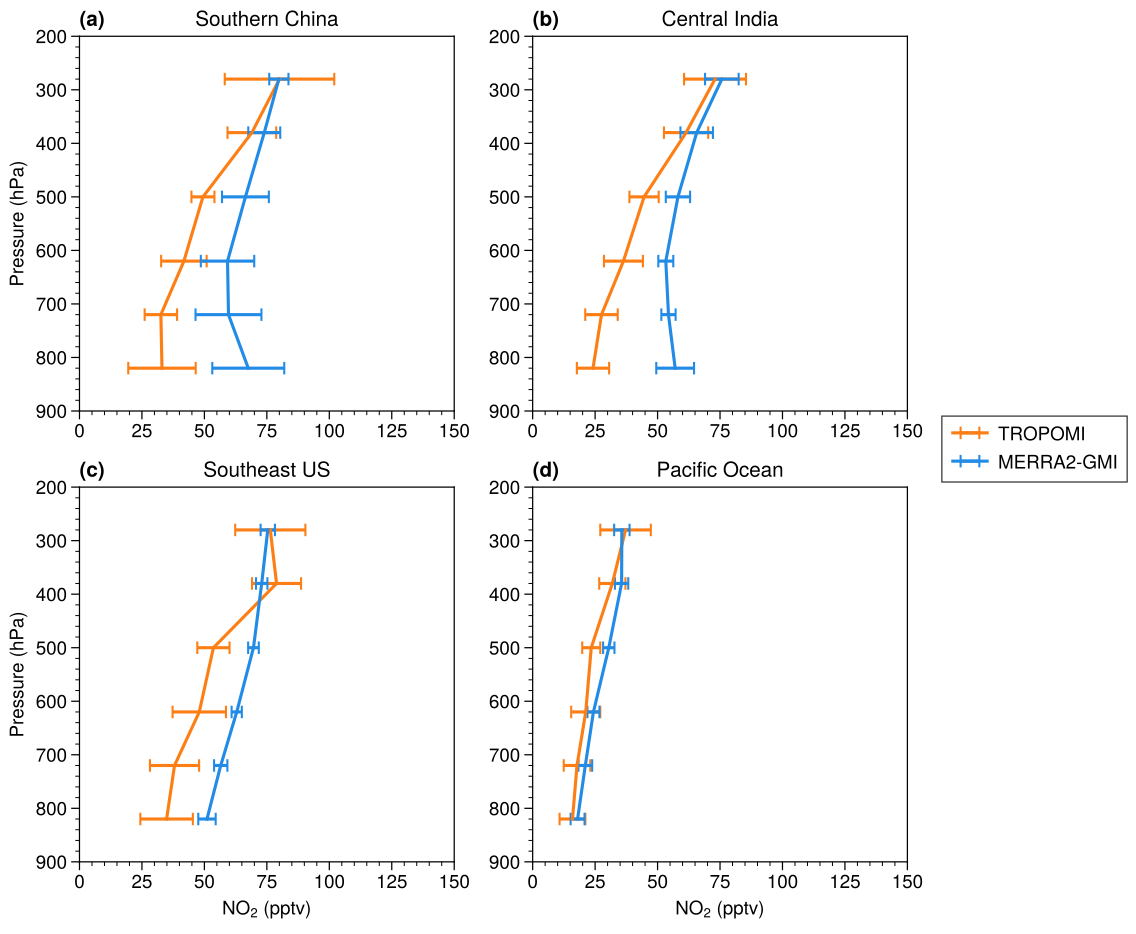
\includegraphics[width=0.9\textwidth]{./figures/uto3_profile.png}
    \caption{
    MERRA2-GMI(蓝色)和TROPOMI云切片算法(橙色)得到的区域平均O$_{\ch{3}}$廓线
    (a)中国南部;(b)印度中部;(c)美国东南部;(d)太平洋(区域示意图见图\ref{fig:no2_ltngcount}a)。
    其中廓线的误差棒为平均值$\pm$标准差。\\
    Figure \ref{fig:uto3_profile}. Regional average NO$_{\ch{2}}$ profiles obtained by MERRA2-GMI (blue) and TROPOMI cloud slice algorithm (orange).
    (a) southern China, (b) central India, (c) southeastern United States, and (d) Pacific Ocean
    (Definitions of region are shown in Fig. \ref{fig:no2_ltngcount}a).
    The error bars are the mean values $\pm$ standard deviations.
    }
    \label{fig:uto3_profile}
\end{figure}

\begin{figure}[H]
\centering
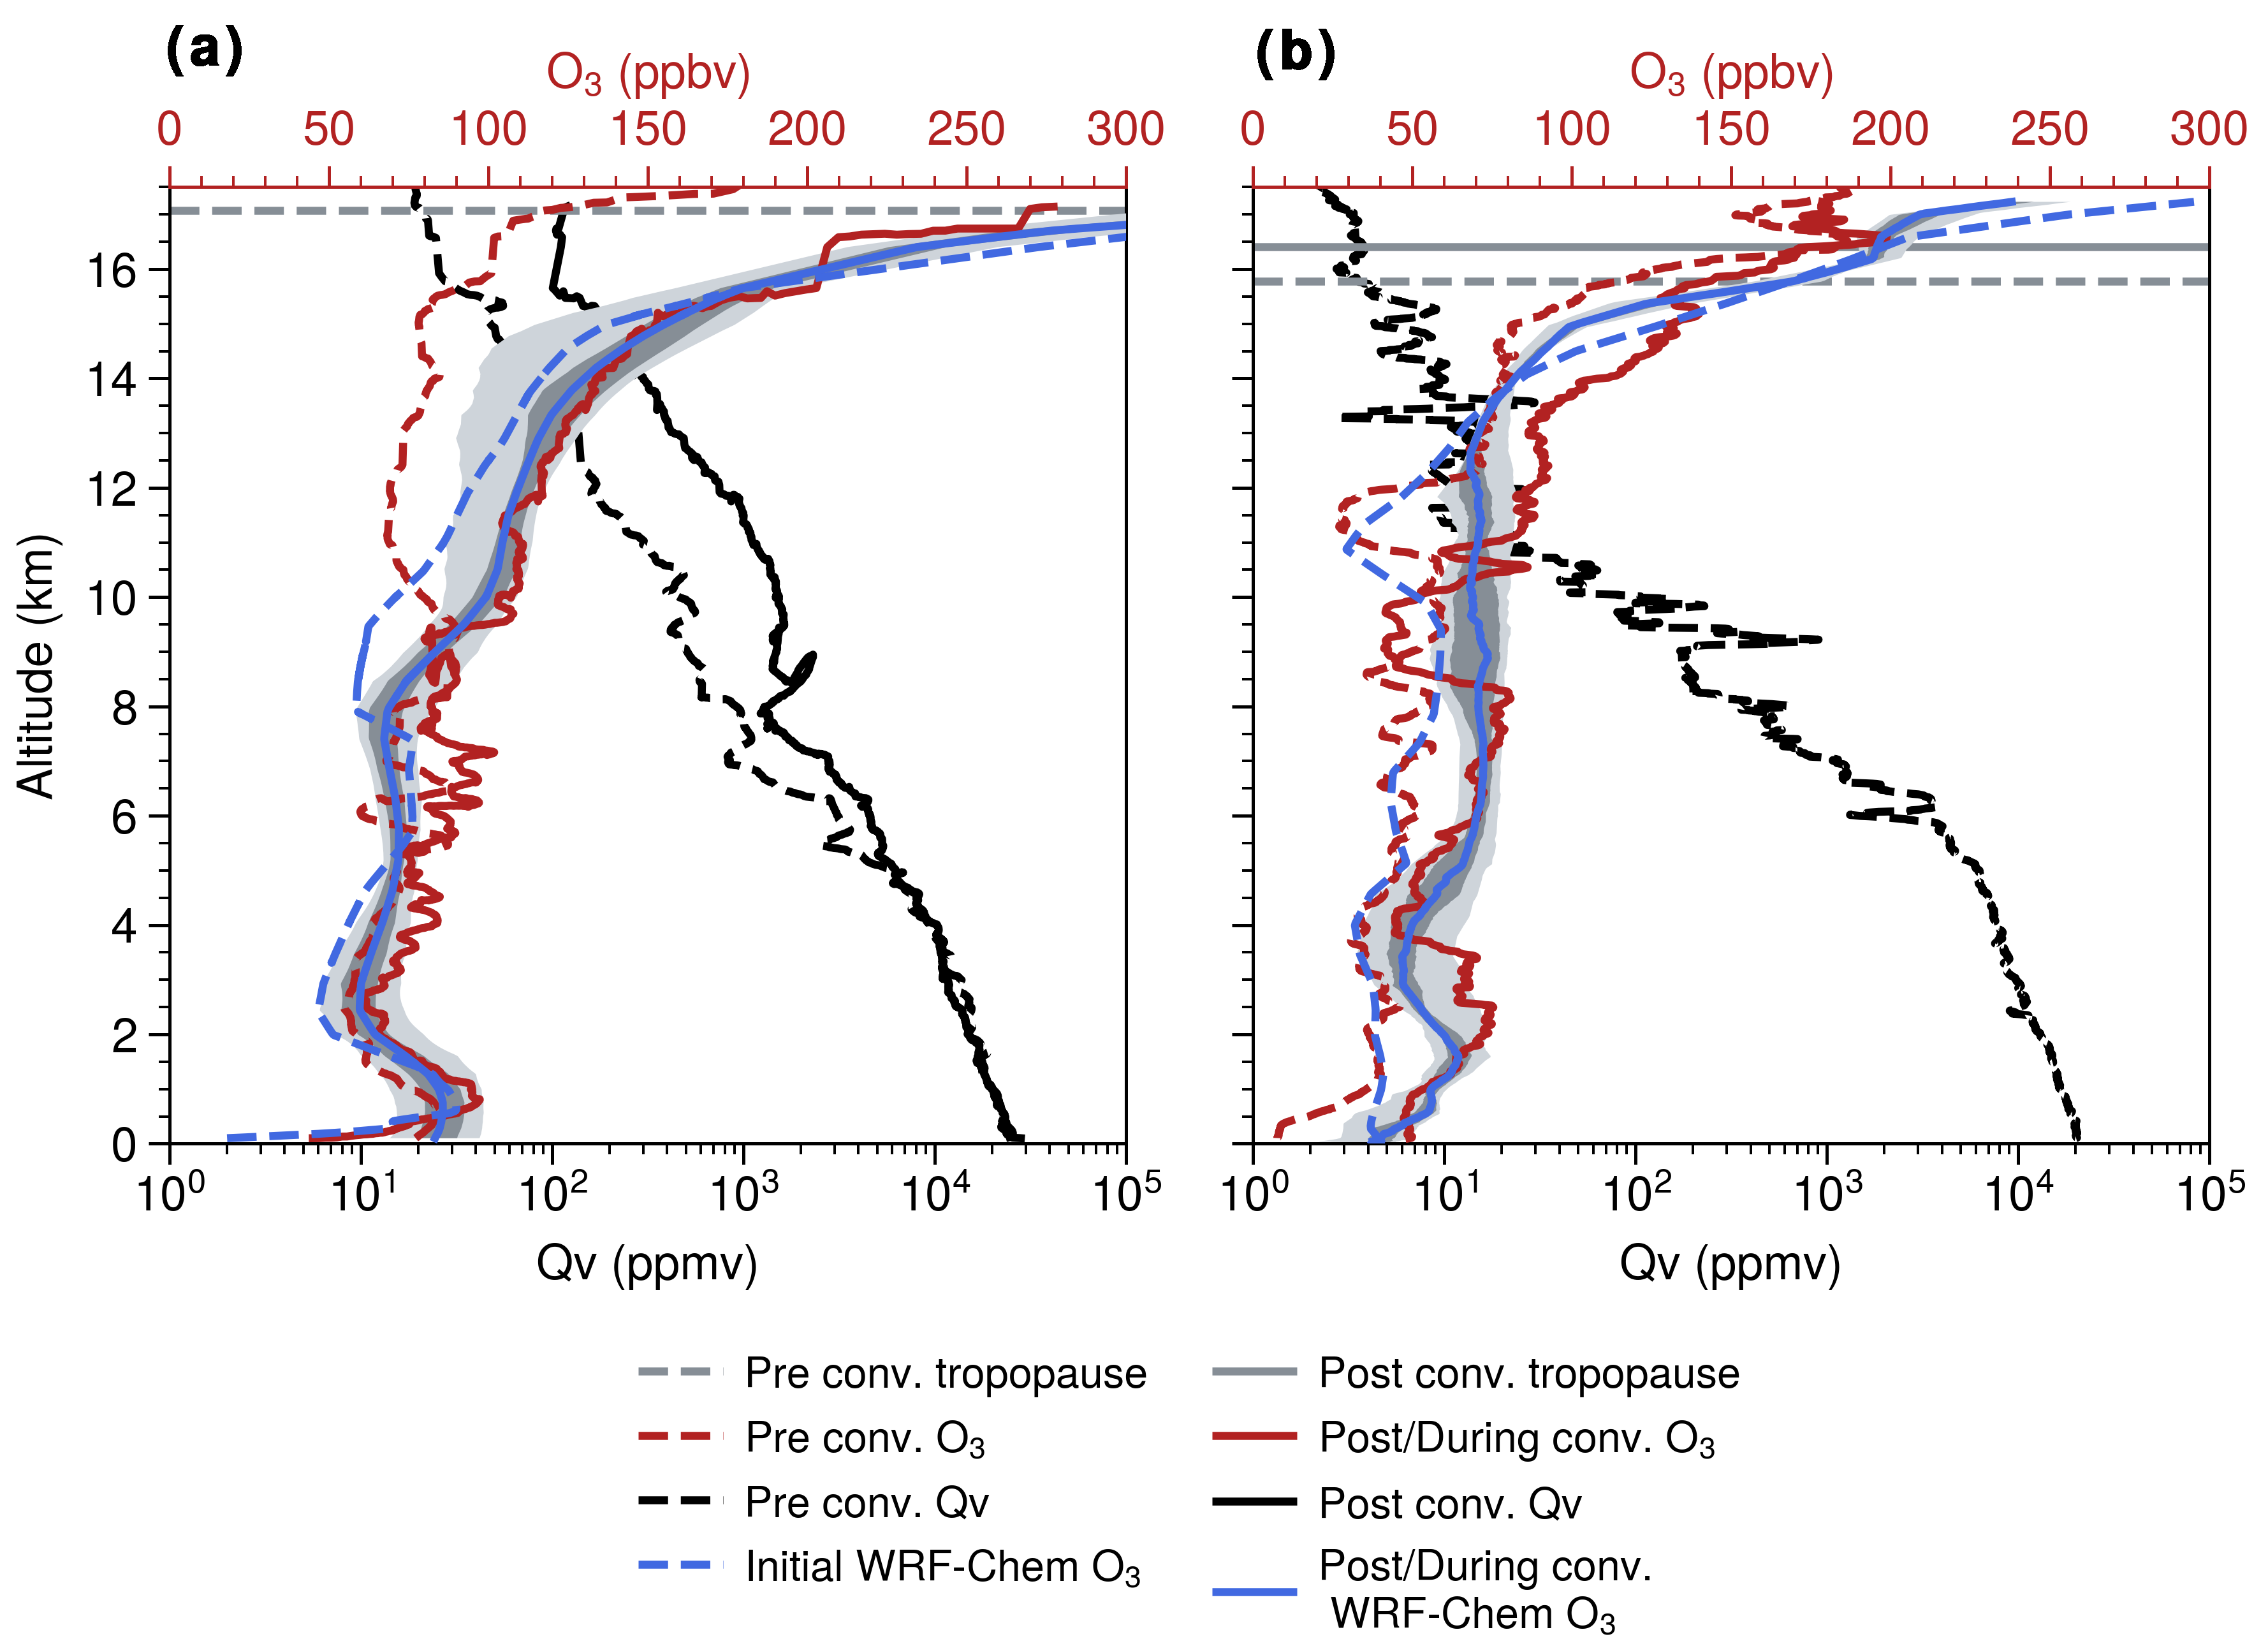
\includegraphics[width=0.9\textwidth]{./figures/ozonesonde_profile.png}
\caption{对流前(虚线)和对流后/对流期间(实线)探空观测到的O$_{\ch{3}}$(红色)和Q$_v$(黑色)廓线。
模式初始(虚线)和对流后或对流期间(实线)的O$_{\ch{3}}$廓线为蓝色。
深灰色阴影是50\%的置信区间,浅色是90\%的置信区间,灰线是第一对流层顶。
(a)2019年个例;(b)2020年个例。\\
Figure \ref{fig:ozonesonde_profile}. Observed O$_{\ch{3}}$ (red) and Q$_v$ (black) profiles in the pre-convection (dashed) and post-convection/during-convection (solid) periods.
The initial (dashed) and simulated post-convection or during-convection (solid) O$_{\ch{3}}$ profiles are in blue.
The dark gray shading is the 50 \% confidence interval while the light one is the 90 \% confidence interval.
The gray lines are the lapse rate tropopauses.
(a) 2019 case and (b) 2020 case.
}
\label{fig:ozonesonde_profile}
\end{figure}

除了云切片算法得到的全球O$_{\ch{3}}$分布外,
中国东南部的臭氧探空试验在对流不同阶段所测得的O$_{\ch{3}}$和Q$_v$分布如图\ref{fig:ozonesonde_profile}所示。
总体来说,对流导致对流层上层O$_{\ch{3}}$和Q$_v$浓度增大,且增强的最大值所在区域居于10--16 km 之间。
% 其中2020年个例的对流层低层(2--8 km)O$_{\ch{3}}$浓度有较大的增加。
两个个例均存在双谷形的O$_{\ch{3}}$廓线,但高度不同:2019年的热对流个例为2 和8 km,2020年的飑线为4 和10 km。
尽管WRF-Chem模式倾向于低估2019年个例对流层下层和2020年个例对流层上层中的O$_{\ch{3}}$浓度,
但仍再现了详细的O$_{\ch{3}}$垂直分布,故能用以分析对流影响O$_{\ch{3}}$的机制。
其中共有三个来源可以解释对流层上层O$_{\ch{3}}$的增加:对流输送、化学反应和闪电直接产生的O$_{\ch{3}}$。
\ref{sec:convec_impacts}节仅详细讨论前两个因素,因为闪电直接产生的O$_{\ch{3}}$
产量仍不确定\citep{Morris.2010,Ripoll.2014}.



\subsection{动力输送和化学反应的贡献} \label{sec:convec_impacts}

为了探究中国东南部对流后对流层上层O$_{\ch{3}}$浓度增大的原因,我们将对流分为三个阶段(初生、发展和消散)来分析臭氧探空仪所经区域中O$_{\ch{3}}$平均浓度的垂直分布廓线变化(图\ref{fig:tendency_o3}a,d)。
其中,2020年个例的对流层上层O$_{\ch{3}}$在整个周期内一直在增加,而2019年个例由于发展阶段低浓度O$_{\ch{3}}$空气的抬升,O$_{\ch{3}}$浓度降低,接着又开始增大,这种现象可以用发展阶段的O$_{\ch{3}}$垂直剖面来解释(图\ref{fig:tendency_o3}b),
低O$_{\ch{3}}$浓度的空气块通过上升气流达到16 km,然后对流后方的高O$_{\ch{3}}$浓度空气被夹卷进该区域。
而2020年个例中观测到增加的O$_{\ch{3}}$,主要来自垂直传输的背景O$_{\ch{3}}$浓度(图\ref{fig:tendency_o3}e)。

\begin{figure}[H]
\centering
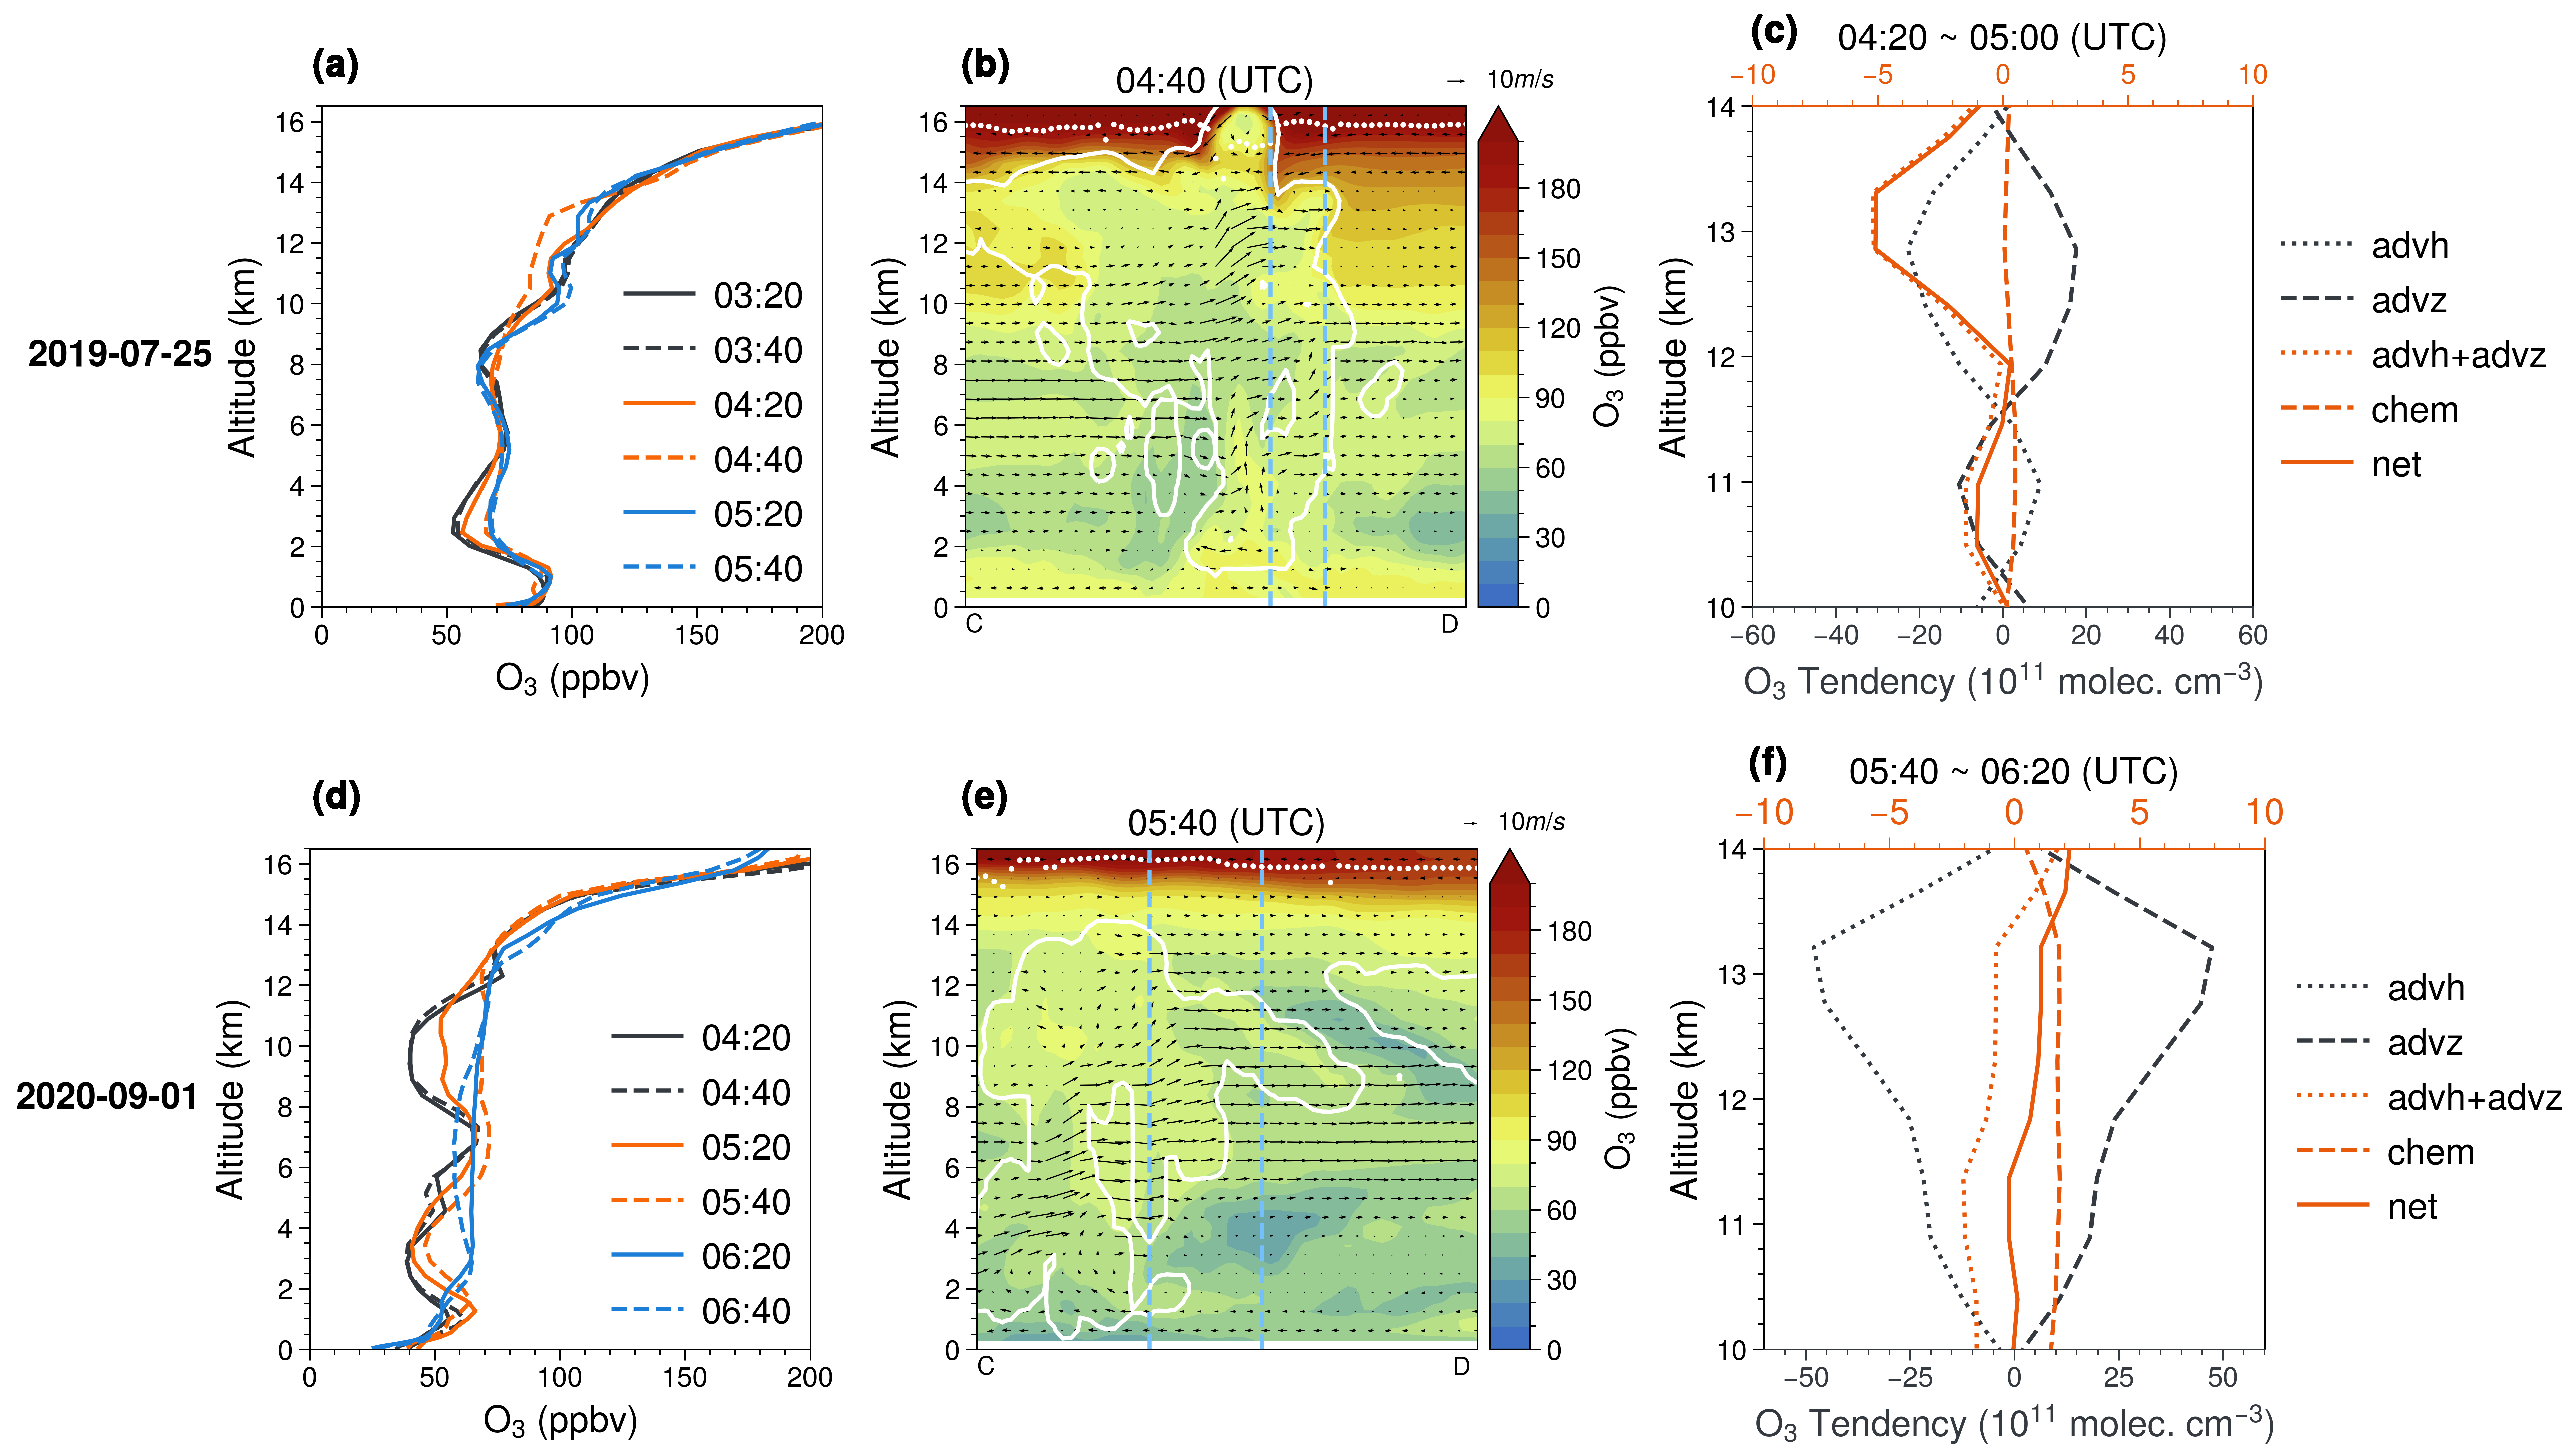
\includegraphics[width=\textwidth]{./figures/tendency_o3.png}
\caption{
(a, d)臭氧探空仪所经区域内的O$_{\ch{3}}$平均浓度剖面,包括三个阶段:初生(黑色)、发展(橙色)和消散(蓝色);
(b,e)对流旺盛期间沿穿过对流核心(图 \ref{fig:comp_crf_2019}e 和图 \ref{fig:comp_crf_2020}f)的O$_{\ch{3}}$剖面。
蓝色虚线代表臭氧探空仪经过区域的边界,第一对流层顶显示为白点。
白线为云边界[云液态水混合比(q$_{cloud}$)和冰混合比(q$_{ice}$)之和 $\geq$ 0.01 g/kg];
(c, f)对流旺盛期的水平平流(advh)、垂直平流(advz)和化学贡献(chem)引起的O$_{\ch{3}}$净产率和趋势的垂直分布。
\\
Figure \ref{fig:tendency_o3}. (a, d) The mean O$_{\ch{3}}$ profiles in the regions passed by the ozonesondes
at three stages: initiation (black), development (orange), and dissipation (blue).
(b, e) Vertical O$_{\ch{3}}$ distribution within the convective periods along the line crossing the convective core (Fig. \ref{fig:comp_crf_2019}e and Fig. \ref{fig:comp_crf_2020}f).
The blue dashed lines stand for the boundaries of regions passed by the ozonesondes, and the lapse rate tropopause is shown as the white dots.
The cloud boundaries [the sum of cloud liquid water mixing ratio (q$_{cloud}$) and ice mixing ratio (q$_{ice}$) $\geq$ 0.01 g/kg] are shown in white lines.
(c, f) The vertical distributions of the O$_{\ch{3}}$ net production rate and tendency due to horizontal advection (advh), vertical (advz) advection, and chemistry (chem) during the convective periods.
}
\label{fig:tendency_o3}
\end{figure}

为了确定两种影响之间的差异,我们分析了对流期间10--14 km的平均累积物理变化速率(IPR,图\ref{fig:tendency_o3}c,f)。
其中水平平流(advh)和垂直平流(advz)的相反趋势支配着2019年对流层上层O$_{\ch{3}}$产率的下降。
由于强上升气流使得低O$_{\ch{3}}$浓度的空气块得以抬升,故垂直平流(advz)的贡献在10--11.5 km之间为负,而在11.5到13.8km 之间为正,即存在向下输送的高浓度O$_{\ch{3}}$空气块。
由于2020年对流个例发生后的Q$_v$较高(图\ref{fig:ozonesonde_profile}a)且对流层顶高于云区(图\ref{fig:tendency_o3}b),
所以其上升气流不足以像中尺度对流系统一样将平流层高浓度的O$_{\ch{3}}$挟至对流层\citep{Phoenix.2020}。
虽然动力输送在O$_{\ch{3}}$的变化中起着重要作用,但不能忽视正的化学贡献,尤其是2020年对流期间化学贡献造成对流层上层O$_{\ch{3}}$的净增加。
具体来说,在两次个例整个生命期中化学反应对O$_{\ch{3}}$起到了正贡献,
其影响程度是动力输送的5--10倍,这表明化学贡献在对流的整个生命期中占主导地位。

由以上的中国东南部O$_{\ch{3}}$浓度变化分析可知化学贡献的重要性,
因此我们进一步利用MERRA2-GMI的3小时平均模式结果,分析了动力(大尺度输送)、物理(湍流和对流)和化学对中低纬度O$_{\ch{3}}$的贡献。
如图\ref{fig:uto3_tendency}所示,中低纬度的O$_{\ch{3}}$趋势主要由动力项主导,且噪点较多,
物理的贡献主要为负,代表低O$_{\ch{3}}$浓度的空气向对流层上层输送。
然而在污染地区(如美国东南部、非洲中部、印度北部以及中国东南部)化学贡献的正贡献占主导,表明O$_{\ch{3}}$的净生成。
由于对流和闪电产生较高浓度的NO$_{\ch{2}}$,这些区域的正化学贡献在阴天比晴天高50--160\%(图\ref{fig:uto3_chem_tendency})。
该结果与中国东南部O$_{\ch{3}}$在整个对流生命期的变化及来源相符,突出了LNO$_{\ch{2}}$对于夏季对流层上层O$_{\ch{3}}$浓度的长期影响。


\begin{figure}[H]
    \centering
    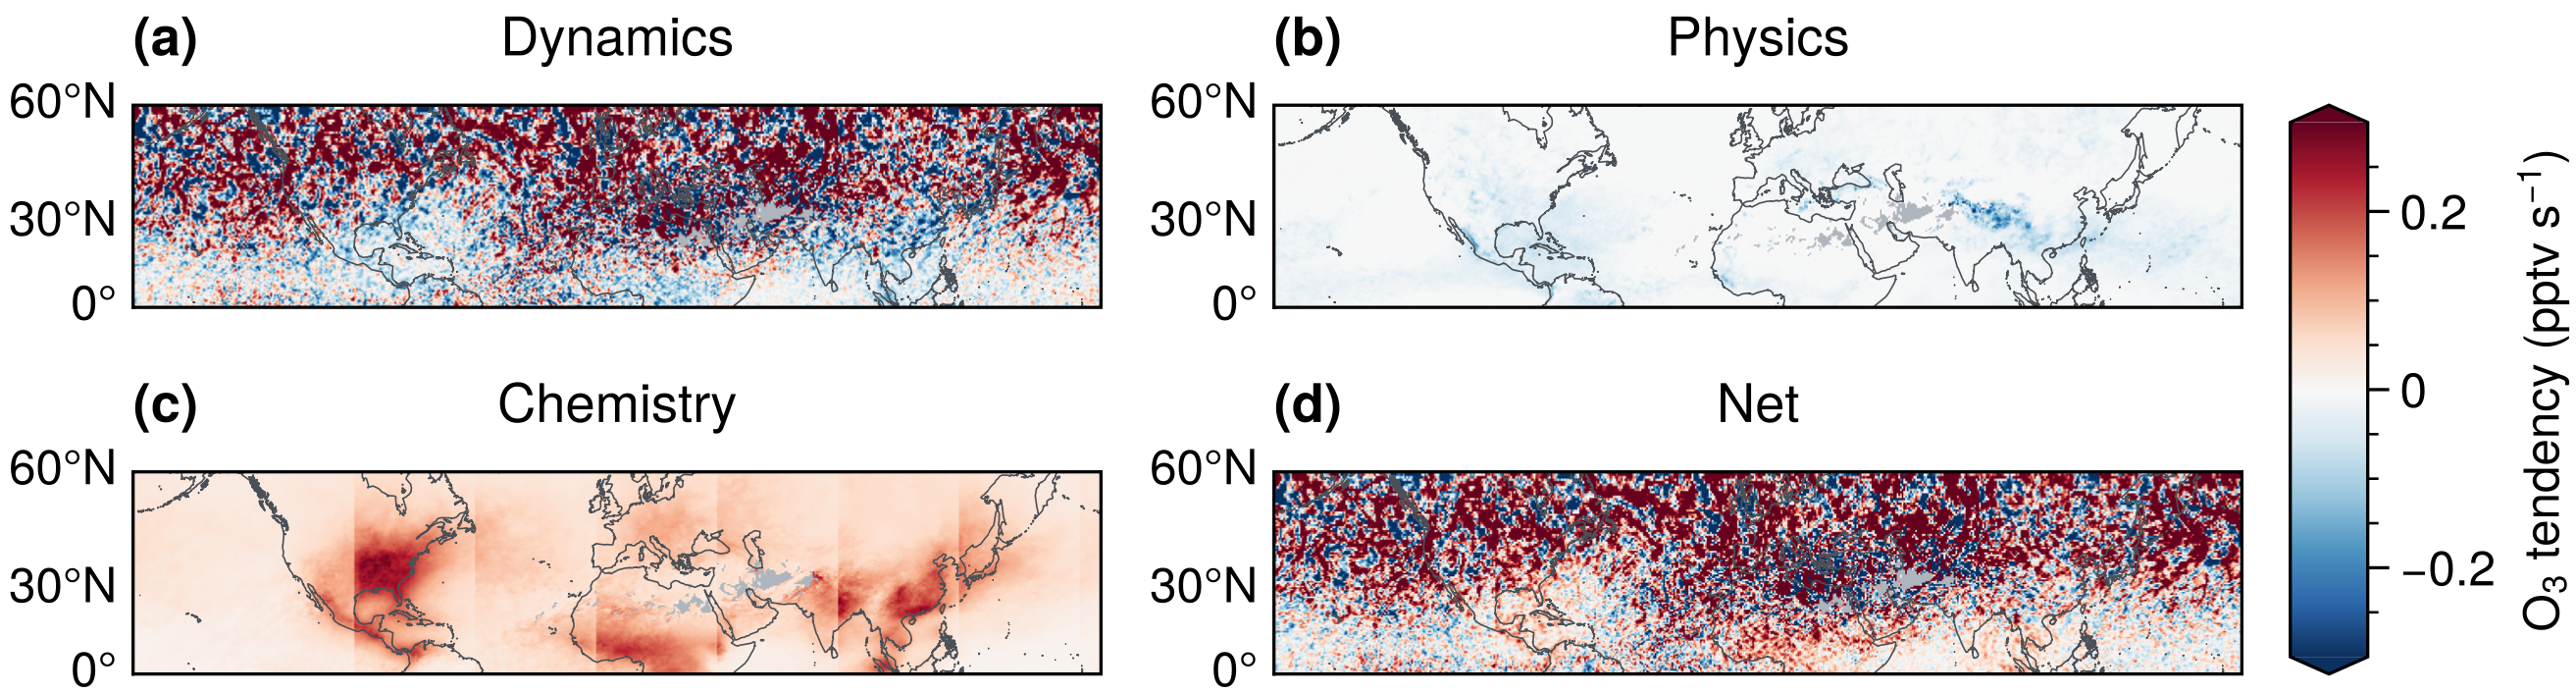
\includegraphics[width=\textwidth]{./figures/uto3_tendency.png}
    \caption{
    2019年6--8月北半球中低纬度MERRA2-GMI模拟的261 hPa高度O$_{\ch{3}}$的平均趋势:
    (a)动力;(b)物理;(c)化学;(d)净趋势。\\
    Figure \ref{fig:uto3_tendency}. The mean tendency of O$_{\ch{3}}$ simulated by MERRA2-GMI at 261 hPa due to (a) dynamics, (b) physics, (c) chemistry, and (d) net tendency at the northern middle-low latitudes for June--August in 2019.
    }
    \label{fig:uto3_tendency}
\end{figure}


\begin{figure}[H]
    \centering
    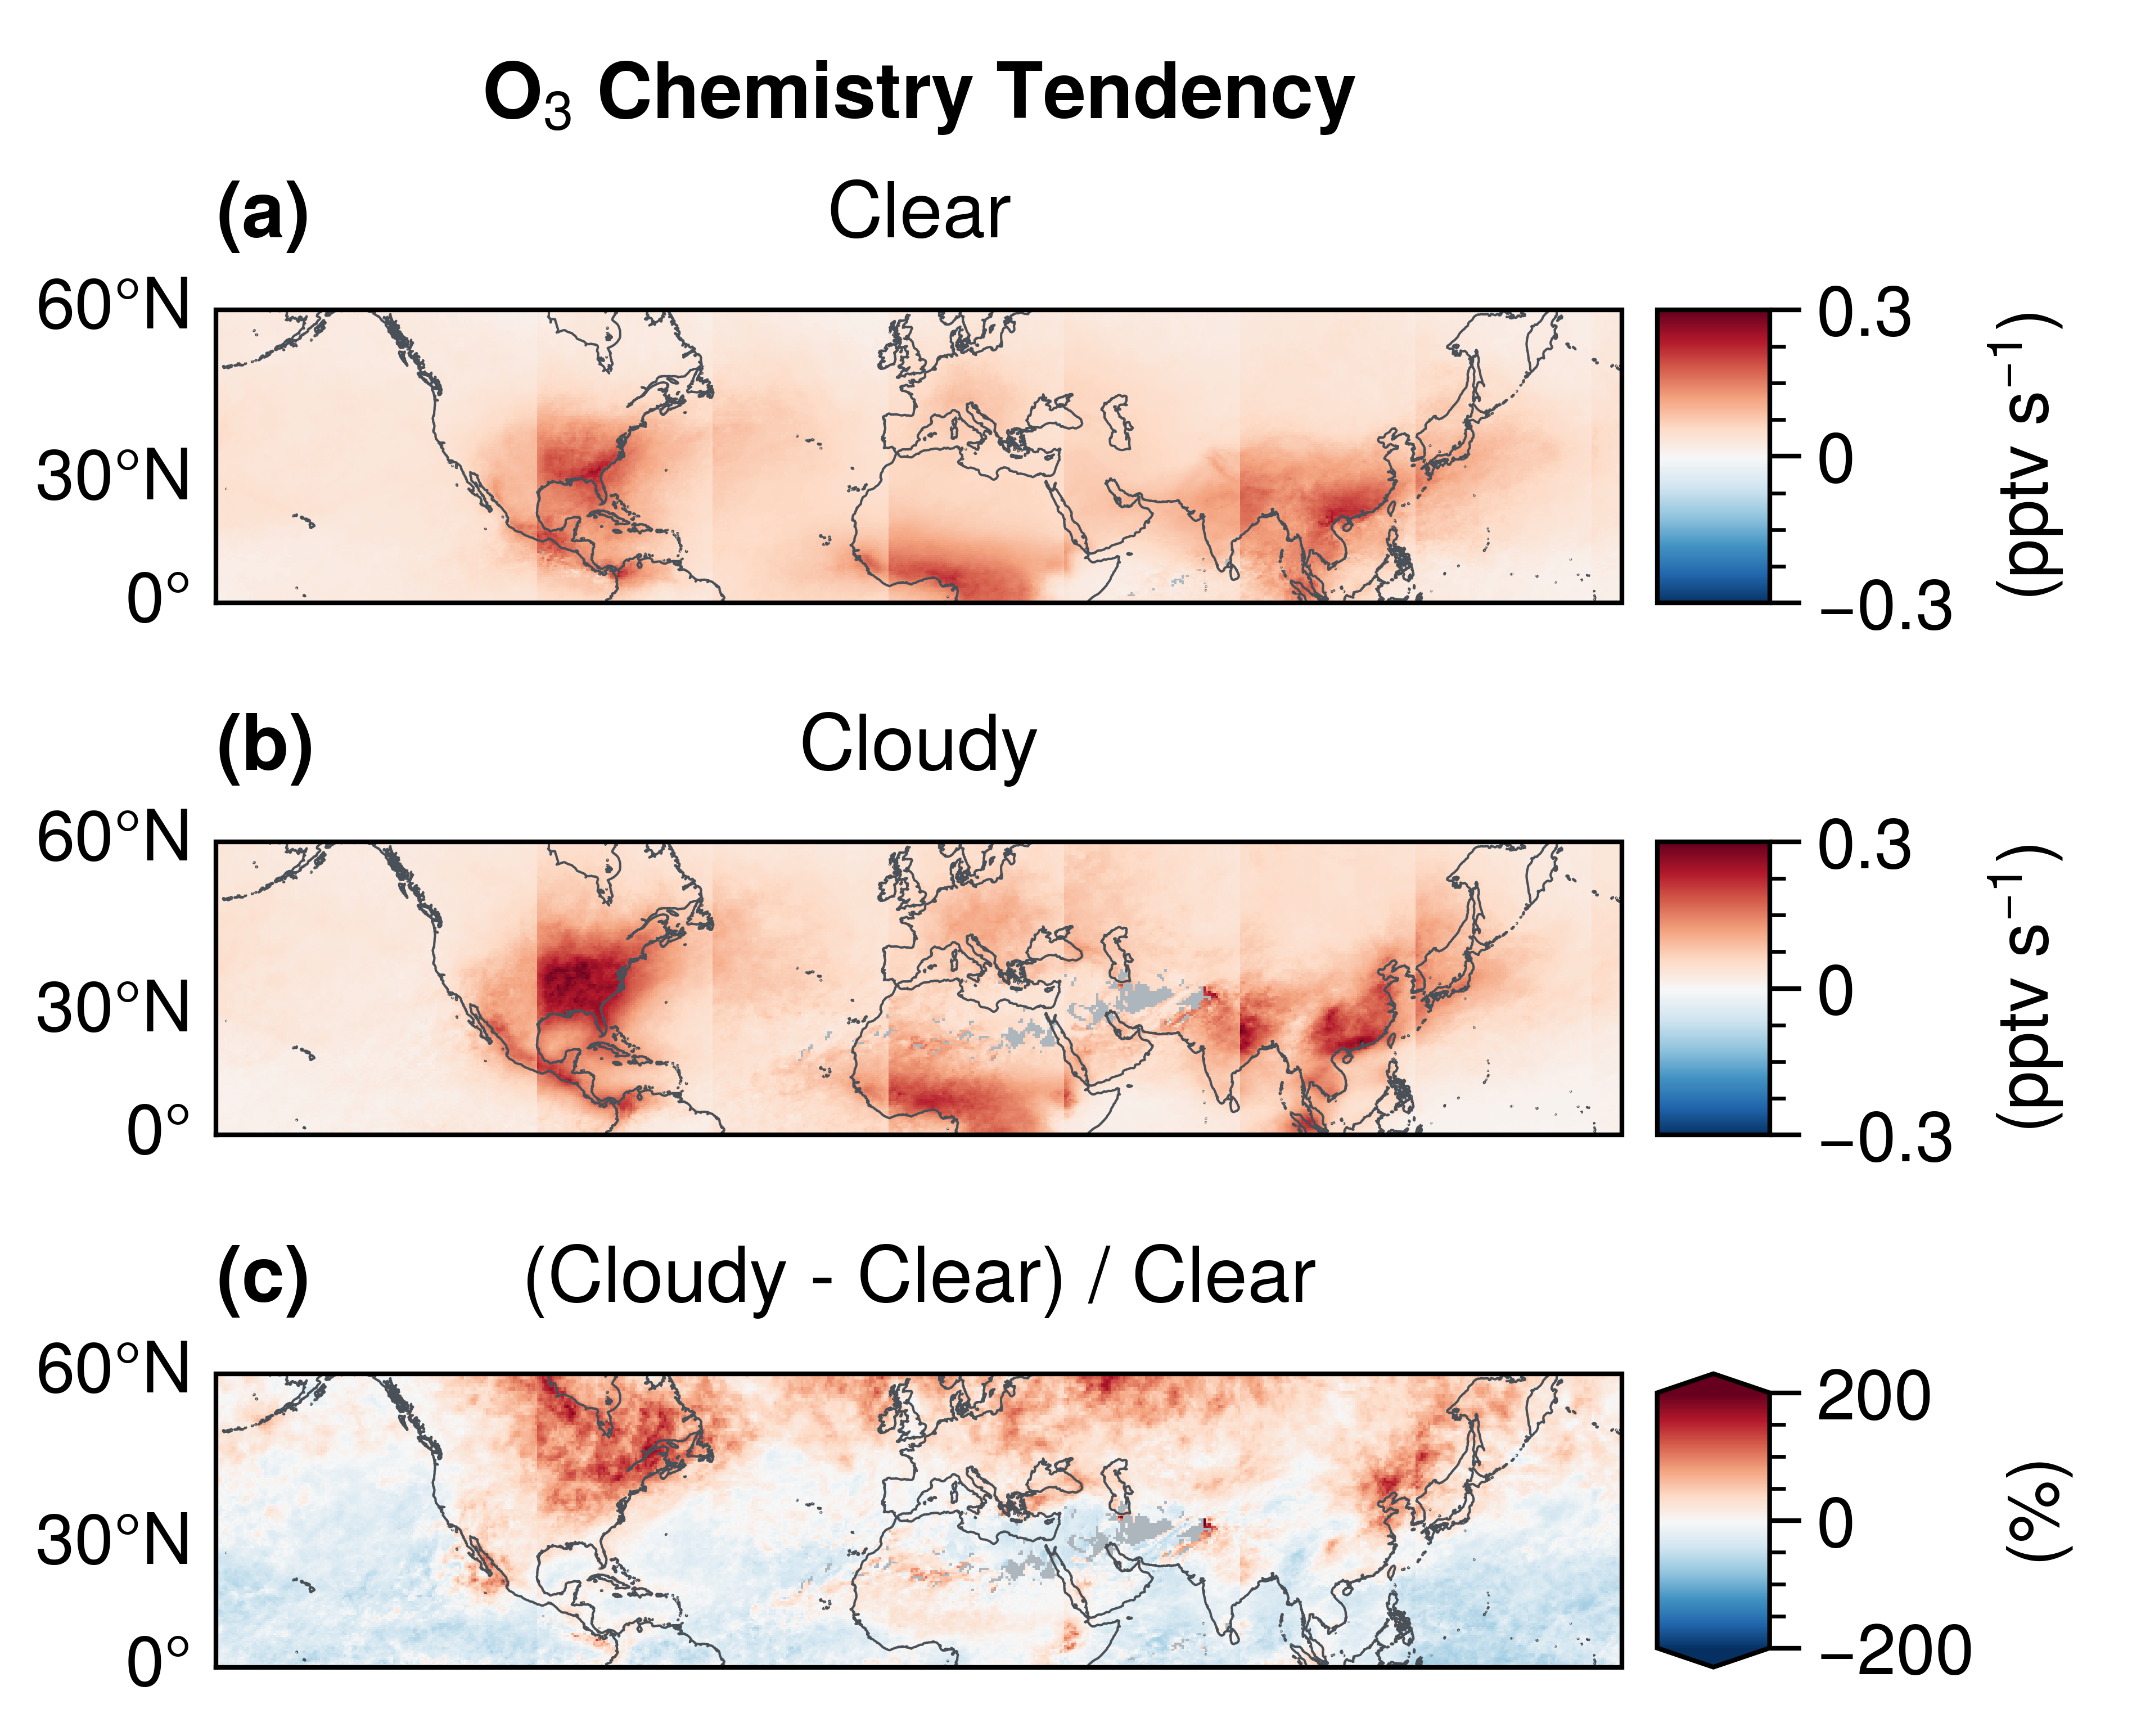
\includegraphics[width=\textwidth]{./figures/uto3_chem_tendency.png}
    \caption{
    2019年6--8月北半球中低纬度MERRA2-GMI模拟的261 hPa高度O$_{\ch{3}}$的平均化学趋势:
    (a)晴空条件;(b)有云条件;(c)两者的相对差。\\
    Figure \ref{fig:uto3_chem_tendency}. The mean chemistry tendency of O$_{\ch{3}}$ simulated by MERRA2-GMI for 261 hPa at the northern middle-low latitudes for June--August in 2019:
    (a) clear condition, (b) cloudy condition, and (c) percentage differences.
    }
    \label{fig:uto3_chem_tendency}
\end{figure}

\subsection{闪电氮氧化物的影响} \label{sec:lnox_effects}

我们将开启和关闭LNO排放所得到的中国东南部O$_{\ch{3}}$累计物理变化速率(IPR)进行对比,
从而得到LNO$_{\ch{x}}$对O$_{\ch{3}}$的影响(表\ref{table:ipr})。
如上节所述,化学的正贡献主导了整个对流生命期间O$_{\ch{3}}$浓度的变化,是对流输送贡献的5--10倍。
在2019年个例的对流旺盛期和整个生命周期中,LNO$_{\ch{x}}$使得O$_{\ch{3}}$的净产量分别降低了25\%和40\%。
而对于2020年个例,由于站点附近闪电密度较小,化学贡献导致的O$_{\ch{3}}$浓度变化不显著($\leq$1 \%)。
% 而前人研究表明,LNO$_{\ch{x}}$在日尺度范围内可提高下风向的O$_{\ch{3}}$产量\citep{Pickering.1996,DeCaria.2005}。
% 因此,有必要准确估计LNO$_{\ch{x}}$的产率(见第\ref{chapter:PE}章)。


\begin{table*}[h]
\centering
\caption{平均O$_{\ch{3}}$累积趋势的过程分析(10--14 km)\\ Table \ref{table:ipr} Process analysis table for the mean O$_{\ch{3}}$ integrated tendencies (10--14 km)}
\footnotesize
{\centering
\renewcommand{\arraystretch}{1}
\begin{tabular}{@{\extracolsep{\fill}} cccccc}
\thickline
  Period           & Time             & LNO (mol/flash) & advh + advz$^a$       & chem$^a$              & net$^a$    \\
\thickline
Life Cycle         & 2019-07-25       & 0               & -3.3 (-24.6 \%)        & 16.7 (124.6 \%)        & 13.4       \\
                   & (03:20--05:40)   & 500             & -2.3 (-28.8 \%)        & 10.3 (128.8 \%)        & 8.0        \\
\cline{2-6}
                   & 2020-09-01       & 0               & 3.4  (9.6 \%)          & 32.0 (90.4 \%)         & 35.4       \\
                   & (04:20--06:40)   & 500             & 4.4  (12.1 \%)         & 31.9 (87.8 \%)         & 36.3       \\
\hline
Convective Period   & 2019-07-25      & 0              & -19.6 (140.0 \%)       & 5.6 (-40.0 \%)         & -14.0      \\
                    & (04:20--05:00)  & 500            & -20.0 (114.3 \%)       & 2.5 (-14.3 \% )        & -17.5      \\
\cline{2-6}
                    & 2020-09-01      & 0              & -9.7  (-131.1 \%)      & 17.1 (231.1 \% )       & 7.4        \\
                    & (05:40--06:20)  & 500            & -10.1 (-148.5 \%)      & 16.9 (248.5 \% )       & 6.8        \\
\thickline
\end{tabular}
\par }
\begin{tablenotes}
\linespread{1}\footnotesize
\item $^{a}$ 单位是 10$^{10}$ molec. cm$^{-3}$。百分比是每种贡献在净O$_{\ch{3}}$变化中的比例。 \\
\item $^{a}$ The unit is 10$^{10}$ molec. cm$^{-3}$. The percentage is the proportion of each part in the net O$_{\ch{3}}$ change.
\end{tablenotes}
\label{table:ipr}
\end{table*}


% 此外,我们利用TROPOMI数据将对流分为三个区域:新生闪电区、闪电下风向和闪电老化区(详见\ref{sec:lnox_affects_tropomi}节和图\ref{fig:china_s5p_amf_diff})。
% 首先基于不同LNO产率的模拟结果,获得O$_{\ch{3}}$差异($\Delta$O$_{\ch{3}}$)的廓线(图\ref{fig:irr_timeseries}a--c)。
% $\Delta$O$_{\ch{3}}$在2--5 km之间大部分为正($<$1 ppbv),在5--12 km 之间为负($>$-3 ppbv),
% 这与\citet{Ott.2007}研究中所有高度上O$_{\ch{3}}$都产生净损失($>$-4 ppbv)的结论不一致。
% 此外,较高的LNO产率(700 mol 每闪电)与默认500 mol 每闪电的结果相比,所有高度的O$_{\ch{3}}$浓度均降低,
% 甚至导致闪电下风向2--5 km高度的$\Delta$O$_{\ch{3}}$由正转负(图\ref{fig:irr_timeseries}b)。
% 由于LNO$_{\ch{x}}$在8--10 km高度达到峰值,O$_{\ch{3}}$浓度也在此层降低最多。%(2.6 ppbv)。

% \setlength{\abovedisplayskip}{3pt} % decrease space before equation
% \setlength{\belowdisplayskip}{3pt} % decrease space after equation
接着,我们以受LNO$_{\ch{2}}$影响更大的2019年为例,利用积分反应速率(IRR)来评估LNO$_{\ch{x}}$对$\Delta$O$_{\ch{3}}$的影响,以及O$_{\ch{3}}$变化的化学机制。
% 我们分两层来看该影响,因为800--500 hPa上$\Delta$O$_{\ch{3}}$为正,500--200 hPa上$\Delta$O$_{\ch{3}}$为负。
对流层O$_{\ch{3}}$主要由以下反应速率项控制\citep{Mazzuca.2016}:
{
\abovedisplayskip=3pt%
\belowdisplayskip=3pt%
\begingroup
\allowdisplaybreaks
\begin{align}
  \frac{d}{dt}[\mathrm{O_3}] &= k_1[\mathrm{NO}][\mathrm{HO_2}] + \sum_{i}  k_i[\mathrm{NO}][\mathrm{R_iO_2}] - k_3[\mathrm{OH}][\mathrm{NO_2}][\mathrm{M}] - P(\mathrm{RONO_2}) \nonumber \\
                             & - k_4[\mathrm{HO_2}][\mathrm{O_3}] - k_5[\mathrm{OH}][\mathrm{O_3}] - k_6[\mathrm{H_2O}][\mathrm{O(^1D)}] - L(\mathrm{O_3+alkenes})
\end{align}
\endgroup
}

其中k$_i$是过氧自由基(R$_i$O$_{\ch{2}}$)与NO之间的反应速率系数,
$P(\ch{RONO2})$为硝酸盐生成反应,
$L(\mathrm{O_3+alkenes})$为烯烃消耗O$_{\ch{3}}$的反应。
由于OH+NO$_{\ch{2}}$、O$_{\ch{3}}$+HO$_{\ch{2}}$和O(1D)+H$_2$O共占O$_{\ch{3}}$化学消耗的85--95\%,
故IRR时间序列图(图\ref{fig:irr_timeseries})除O$_{\ch{3}}$生成反应外,仅包含了此三种消耗反应。
由于2019年对流个例的垂直运动剧烈(见\ref{sec:convec_impacts}节),
故净积分反应速率的时间序列变化可达1.8$\times$10$^7$ molec. cm$^{-3}$ s$^{-1}$,且O$_{\ch{3}}$净化学产量保持正值。
总体而言,整个生命期间LNO$_{\ch{2}}$的排放导致对流层上层O$_{\ch{3}}$化学总生成量降低4\%,
总损耗量增加23\%。
具体而言,NO+HO$_{\ch{2}}$之间的正贡献始终占主导地位(75--80\%),
而另一正贡献即RO$_{\ch{2}}$对NO的氧化占20--25\%,该两种反应的IRR在LNO的作用下,均在对流旺盛期增大$\sim$10\%而后降低$\sim$35\%。
对于O$_{\ch{3}}$的消耗反应而言,对流旺盛期前是O$_{\ch{3}}$+OH和OH+NO$_{\ch{2}}$占主导,且两者速率相当(1--2$\times$10$^6$ molec. cm$^{-3}$ s$^{-1}$),
而由于对流系统中LNO的排放,使得OH 和 HO$_{\ch{2}}$ 之间的平衡向OH方向移动,其中OH+NO$_{\ch{2}}$的IRR是O$_{\ch{3}}$和OH的1.2--2.8倍。


\begin{figure}[H]
\centering
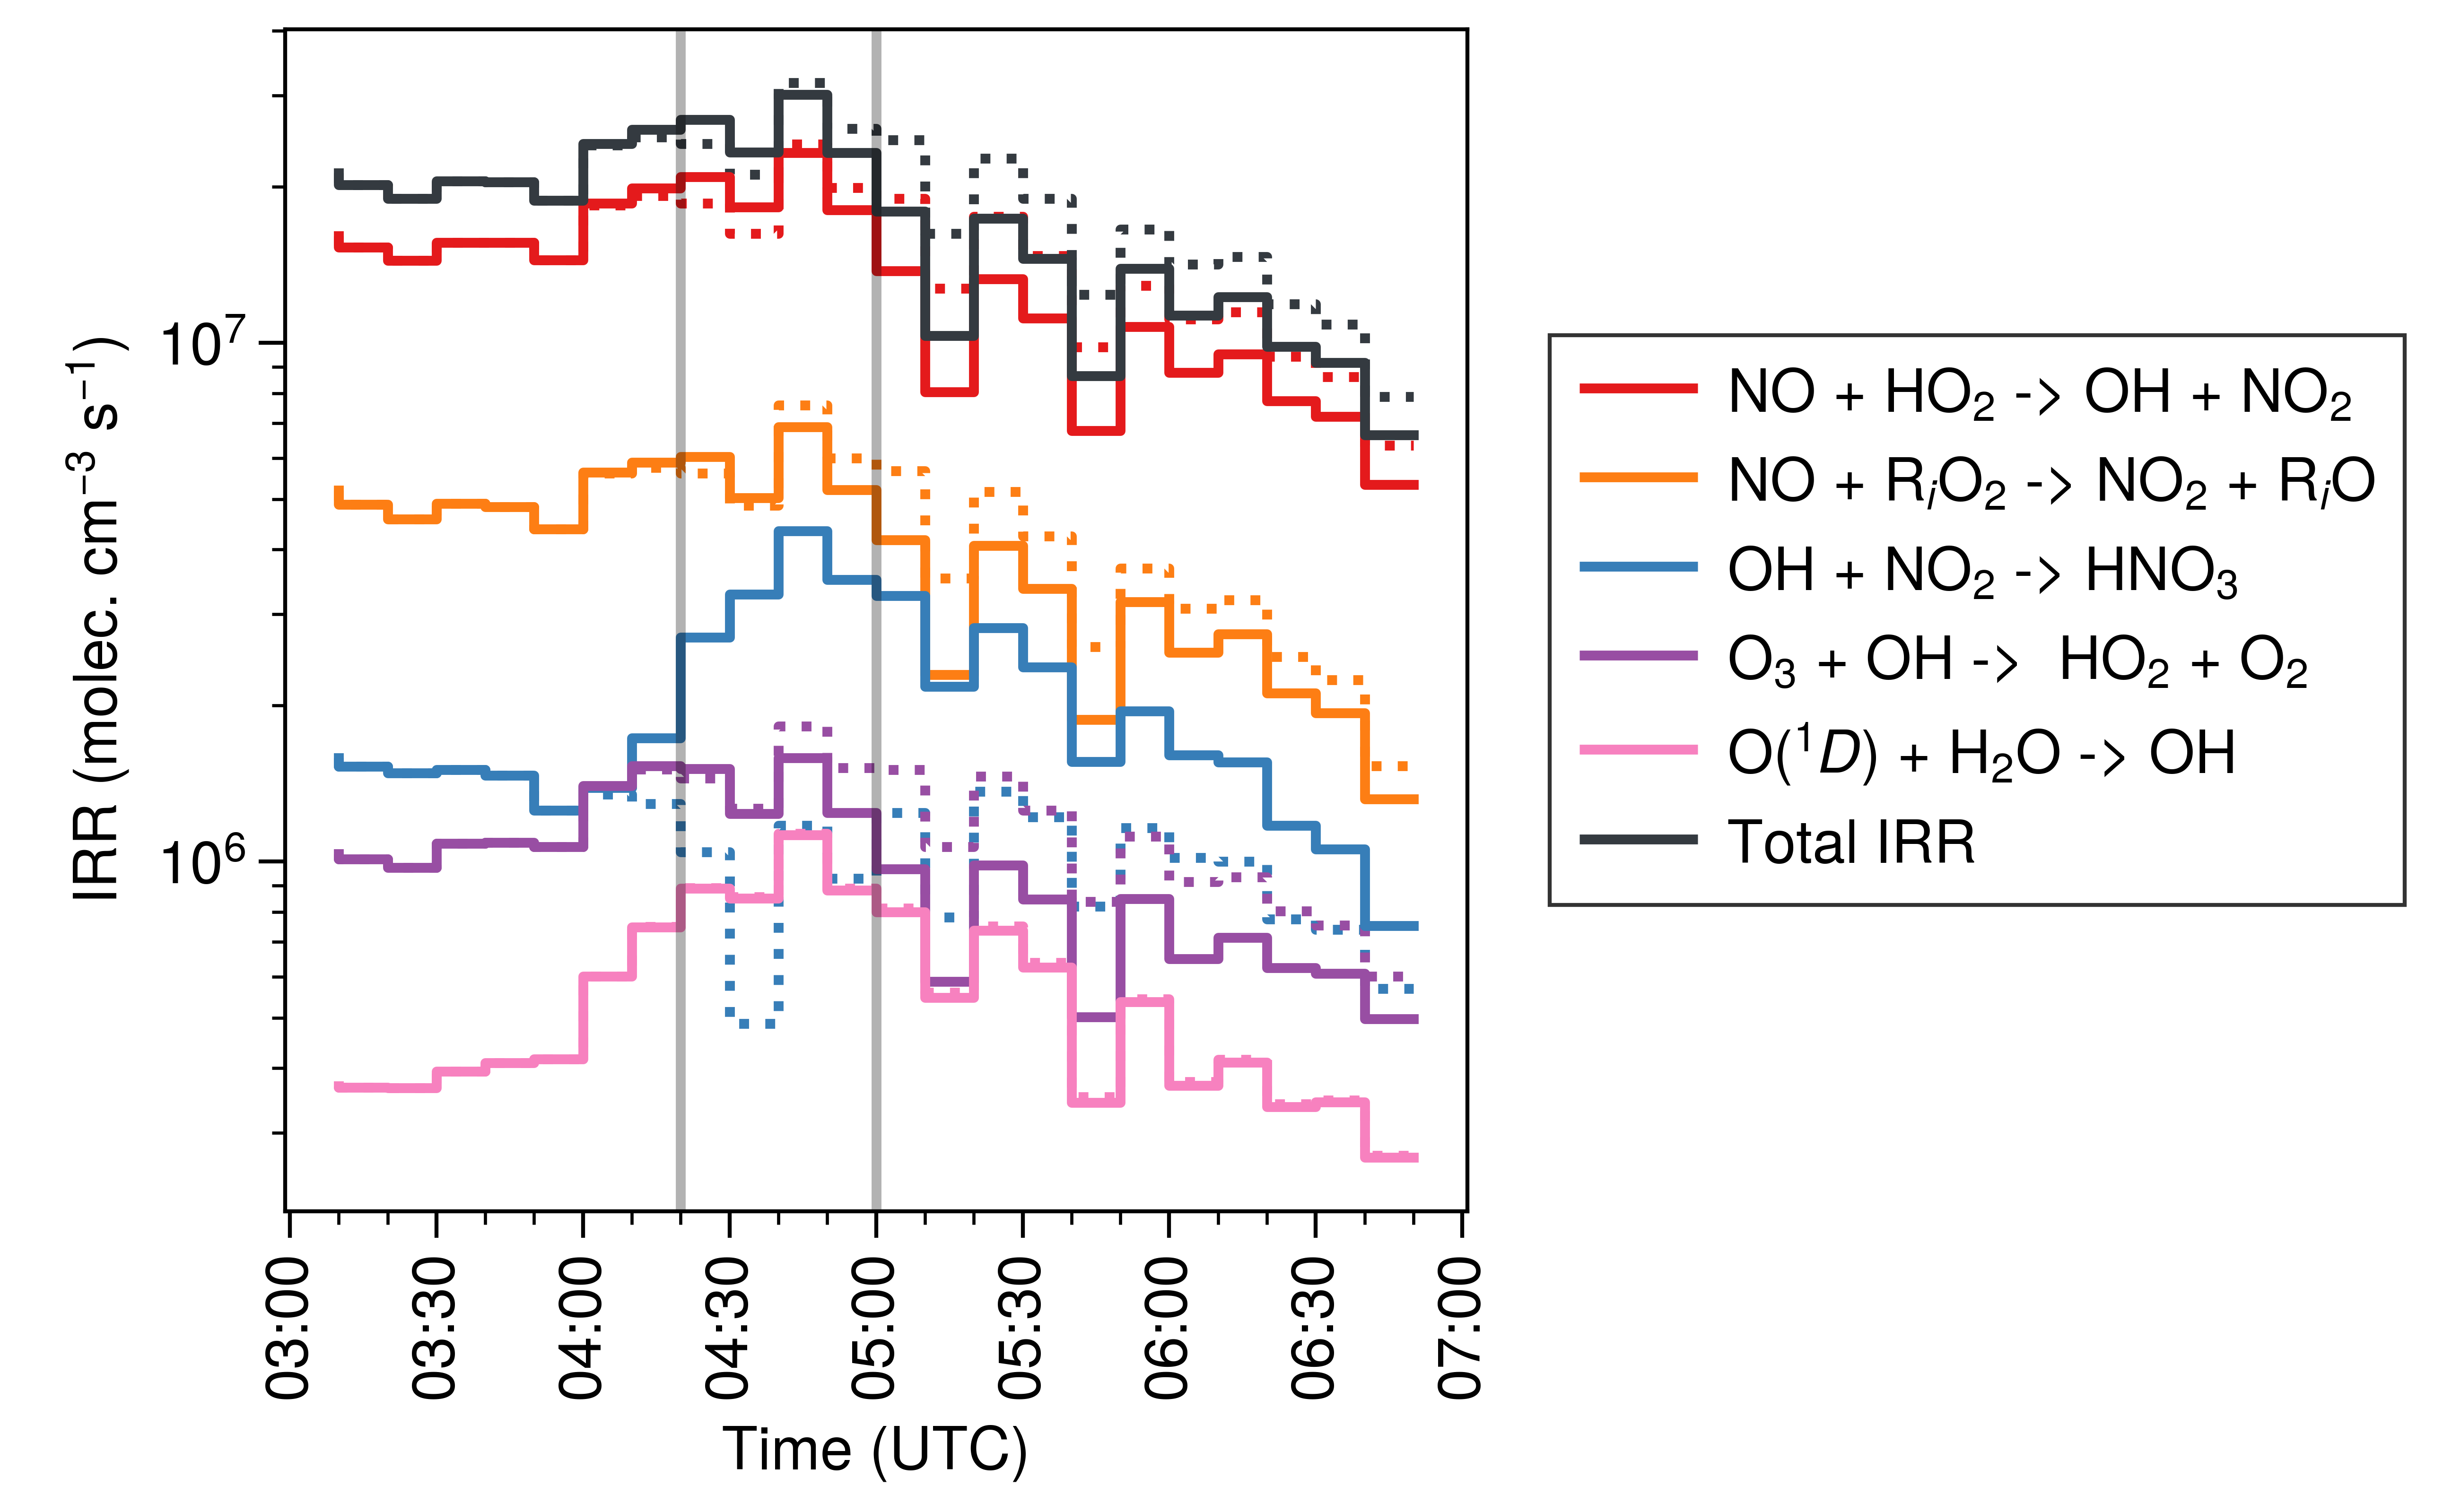
\includegraphics[width=0.9\textwidth]{./figures/irr_timeseries.png}
\caption{
2019年个例中臭氧探空仪所经区域内10--14 km高度间,与O$_{\ch{3}}$有关的主要平均累积反应速率(IRR)的时间序列。
其中图例显示了详细的物种和反应,总IRR是从生成O$_{\ch{3}}$的IRR(红线和橙线)中减去O$_{\ch{3}}$损失的IRR。
实线为模拟中开启LNO(500 mol 每闪电)排放的IRR,而虚线表示关闭LNO排放。\\
Figure \ref{fig:irr_timeseries}. Time series of the mean integrated reaction rate (IRR) of reactions related to O$_{\ch{3}}$ between 10 and 14 km in the region passed by ozonesondes in the 2019 case.
The legend shows detailed species and reactions.
The total IRR is the O$_{\ch{3}}$ loss IRR subtracted from the O$_{\ch{3}}$ production IRR (red and orange lines).
The solid line shows the IRR with LNO (500 mol/flash) while the dashed line is without LNO.
}
\label{fig:irr_timeseries}
\end{figure}


\section{本章小结}

本章不仅将云切片的O$_{\ch{3}}$平均浓度和MLS O$_{\ch{3}}$廓线与MERRA2-GMI模拟结果进行对比分析,
而且将中国东南部对流个例的探空试验与WRF-Chem模式结果相结合,对O$_{\ch{3}}$垂直分布变化的贡献项进行了详细讨论,
主要结论如下:

\begin{enumerate}[label=(\arabic*), labelindent=\parindent, nosep, leftmargin=0pt, widest=0, itemindent=*, topsep=0pt, partopsep=0pt, parsep=0pt]

\item 在低纬地区,TROPOMI、MLS和MERRA2-GMI均显示对流层上层低O$_{\ch{3}}$事件常发生于热带西太平洋,
而非洲中部由于对流输送的边界层高O$_{\ch{3}}$浓度气团,对流层上层O$_{\ch{3}}$在有云条件下浓度较晴空下高20\%。

\item 在中纬地区,TROPOMI的云切片结果较少,MLS和MERRA2-GMI的对流层上层O$_{\ch{3}}$趋势相反:
MERRA2-GMI模拟显示对流层上层O$_{\ch{3}}$浓度在有云时比晴空时浓度低26\%,而MLS观测表明有云时O$_{\ch{3}}$浓度增大24\%,
鉴于MERRA2-GMI与TROPOMI的相近,我们将MLS在261 hPa高度层高估的O$_{\ch{3}}$浓度归因于平流层过度的外推。

% % \item MERRA2-GMI在闪电频发的美国东南部的模拟结果显示,330--450 hPa高度不存在TROPOMI观测到的O$_{\ch{3}}$峰值,
% % 故MERRA2-GMI模拟中对流层上层LNO$_{\ch{2}}$的差异导致了O$_{\ch{3}}$浓度的低估;

% % \item 闪电同化后的WRF-Chem对流模拟结果与观测相符,虽然WRF-Chem模式结果倾向于低估O$_{\ch{3}}$浓度,
% % 但其再现了臭氧探空观测到的垂直分布结构及变化,即对流发生后对流层上层的O$_{\ch{3}}$和Q$_v$均增大;

\item MERRA2-GMI和WRF-Chem的O$_{\ch{3}}$趋势分析结果表明,虽然动力输送项在对流旺盛期间占主导,
但在污染地区化学反应的正贡献在整个生命期更为重要,可达动力输送的5--10倍;
中国东南部的对流个例模拟显示,对流生命期内LNO$_{\ch{x}}$可使得对流层上层O$_{\ch{3}}$
的化学累积生成速率降低4\%,累积消耗速率增加23\%。
最终该层O$_{\ch{3}}$的平均浓度降低了25\%。

\end{enumerate}
